\documentclass{article}
\usepackage[margin=0.6in]{geometry}
\usepackage[utf8]{inputenc}
\usepackage{amsfonts}
\usepackage{amsmath}
\usepackage{amssymb}
\usepackage{enumitem}
\usepackage{float}
\usepackage{algorithm}
\usepackage{mathrsfs}
\usepackage[noend]{algpseudocode}
\usepackage[hidelinks]{hyperref}
\usepackage{fontspec}
\usepackage{graphicx}

% TODO Get rid of table and figure environments wherever possible.

% \setmainfont{Palatino Linotype}
\setmainfont{Charter Roman}

\setcounter{secnumdepth}{0}

\let\emptyset\varnothing
\DeclareMathOperator{\dec}{dec}
\DeclareMathOperator{\ord}{ord}
\DeclareMathOperator{\lcm}{lcm}
\algdef{SE}[DOWHILE]{Do}{doWhile}{\algorithmicdo}[1]{\algorithmicwhile\ #1}%

\newcommand{\angled}[1]{\langle#1\rangle}

\author{Otavio Macedo}
\title{A Book of Abstract Algebra - solutions to exercises}

\begin{document}

\maketitle

\tableofcontents

\section{Chapter 2}
\subsection{Set A}
\begin{enumerate}
\item $a * b = \sqrt{|ab|}$ on the set $\mathbb{Q}$. This is not an operation on $\mathbb{Q}$. Square roots have two real solutions, some of them irrational. So, this operation is neither unique nor closed under $\mathbb{Q}$.

\item $a * b = a \ln b$, on the set ${x \in \mathbb{R}},\ x > 0$. This is not an operation because it's not closed. For instance, if $b = 1$ then $a\ln b = 0$, which does not belong to the set above.

\item $a * b$ is a root of the equation $x^2 - a^2b^2 = 0$, on the set $\mathbb{R}$. This is not an operation, since $a * b = \pm ab$, hence not unique.

\item Subtraction, on the set $\mathbb{Z}$. This is an operation.

\item Subtraction, on the set ${n \in \mathbb{Z} : n \geq 0}$. This is not an operation, since a subtraction of non-negative integers may result in a negative integer (not closed under the set).

\end{enumerate}

\subsection{Set B}

\begin{enumerate}
\item $x * y = x + 2y + 4$. Commutative: no; Associative: no; Identity: no; Inverses: no.
\begin{enumerate}[label=(\roman*)]
    \item $0 * 1 = 6$ and $1 * 0 = 5$.
    \item $x * (y * z) = x + 2y + 4z + 12$. $(x * y) * z = x + 2y + 2z + 4$.
    \item $x * e = x \Rightarrow x + 2e + 4 = x \Rightarrow 2e + 4 = 0 \Rightarrow e = -2$. But this value of $e$ does not satisfy the equation $e * y = y$, since $-2 * y = -2 + 2y + 4 = 2y + 2 \ne y$.
    \item No identity implies no inverses.
\end{enumerate}

\item $x * y = x + 2y - xy$. Commutative: no; Associative: no; Identity: no; Inverses: no.
\begin{enumerate}[label=(\roman*)]
    \item $0 * 1 = 2$ and $1 * 0 = 1$.
    \item $(x * y) * z = 2y - xy - 2z - 2yz + xyz$ and $x * (y * z) = x + 2y + 4z - 2yz - xy - 2xz + xyz$.
    \item $x * e = x \Rightarrow x + 2e - xe = x \Rightarrow 2e - xe = 0 \Rightarrow e = 0$. But this value of $e$ does not satisfy the equation $e * y = y$, since $0 * y = 2y \ne y$.
    \item No identity implies no inverses.
\end{enumerate}

\item $x * y = |x + y|$.  Commutative: yes; Associative: no; Identity: yes; Inverses: yes.
\begin{enumerate}[label=(\roman*)]
    \item $|x + y| = |y + x|$.
    \item $||1 + -3| + -5| = 3$. But $|1 + |-3 + -5|| = 9$.
    \item $x * e = x \Rightarrow |x + e| = x \Rightarrow e = 0$. Being commutative, $x * e = e * x$. So $0$ is the identity.
    \item $x * x' = 0 \Rightarrow |x + x'| = 0 \Rightarrow x' = -x$. So, the inverse of $x$ is $-x$.
\end{enumerate}

\item $x * y = |x - y|$.   Commutative: yes; Associative: no; Identity: yes; Inverses: yes.
\begin{enumerate}[label=(\roman*)]
    \item $x - y = -(y - x) \Rightarrow |x - y| = |-(y - x)| = |y - x|$.
    \item $||1 - 3| - 5| = 3$. But $|1 - |3 - 5|| = 1$.
    \item $x * e = x \Rightarrow |x - e| = x \Rightarrow e = 0$. Being commutative, $x * e = e * x$. So $0$ is the identity.
    \item $x * x' = 0 \Rightarrow |x - x'| = 0 \Rightarrow x' = x$. So every element is its own inverse.
\end{enumerate}

\item $x * y = xy + 1$. Commutative: yes; Associative: no; Identity: no; Inverses: no.
\begin{enumerate}[label=(\roman*)]
    \item $xy + 1 = yx + 1$.
    \item $(x * y) * z = xyz + z + 1$. But $x * (y * z) = xyz + x + 1$.
    \item $x * e = x \Rightarrow xe + 1 = x$, which does not have a real solution.
    \item No identity implies no inverses.
\end{enumerate}

\item $x * y = \max\ \{x, y\}$. Commutative: yes; Associative: yes; Identity: no; Inverses: no.
\begin{enumerate}[label=(\roman*)]
    \item $\max\ \{x, y\} = \max\ \{y, x\}$.
    \item $\max\ \{x, \max\ \{y, z\}\} = \max\ \{\max\ \{x, y\}, z\}$.
    \item $x * e = x$ would imply that there exists an $e$ that is smaller than any $x \in \mathbb{R}$, which is false.
    \item No identity implies no inverses.
\end{enumerate}
\end{enumerate}

\subsection{Set C}
Table \ref{tab:binary-operations} lists all the operations for the set $\{a, b\}$. 

\begin{table}[]
    \centering         
    \begin{tabular}{cc|cccccccccccccccc}
    $x$ & $y$ & $O_1$ & $O_2$ & $O_3$ & $O_4$ & $O_5$ & $O_6$ & $O_7$ & $O_8$ & $O_9$ & $O_{10}$ & $O_{11}$ & $O_{12}$ & $O_{13}$ & $O_{14}$ & $O_{15}$ & $O_{16}$ \\
    $a$ & $a$ & $a$     & $a$     & $a$     & $a$     & $a$     & $a$     & $a$     & $a$     & $b$     & $b$      & $b$      & $b$      & $b$      & $b$      & $b$      & $b$      \\
    $a$ & $b$ & $a$     & $a$     & $a$     & $a$     & $b$     & $b$     & $b$     & $b$     & $a$     & $a$      & $a$      & $a$      & $b$      & $b$      & $b$      & $b$      \\
    $b$ & $a$ & $a$     & $a$     & $b$     & $b$     & $a$     & $a$     & $b$     & $b$     & $a$     & $a$      & $b$      & $b$      & $a$      & $a$      & $b$      & $b$      \\
    $b$ & $b$ & $a$     & $b$     & $a$     & $b$     & $a$     & $b$     & $a$     & $b$     & $a$     & $b$      & $a$      & $b$      & $a$      & $b$      & $a$      & $b$     
    \end{tabular}
    \caption{Operations on $\{a, b\}$}
    \label{tab:binary-operations}
\end{table}

\begin{enumerate}
    \item Commutative: $\{O_1, O_2, O_7, O_8, O_9, O_{10}, O_{15}, O_{16}\}$.
    \item Associative: $\{O_1, O_2, O_4, O_6, O_7, O_8, O_{10}, O_{16}\}$.
    \item Identity: $\{O_2, O_7, O_8, O_{10}\}$.
    \item Inverses: $\{O_7, O_{10}\}$.
\end{enumerate}

\subsection{Set D}
\begin{enumerate}
    \item Let $a, b, c \in A^*$. Then:
        $$(ab)c = (a_1\ldots a_mb_1\ldots b_n)c_1\ldots c_p = a_1\ldots a_m(b_1\ldots b_nc_1\ldots c_p) = a(bc)$$
    \item Let $A = \{0, 1\}$ and $a = 001$ and $b = 110$, $a, b \in A^*$. Then $ab = 001110$ and $ba = 110001$, clearly showing that $ab \ne ba$.
    \item Let $a\lambda = \lambda a = a$. So $\lambda$ is the identity for this operation.
\end{enumerate}

\section{Chapter 3}

\subsection{Set A}

\begin{enumerate}
    \item $x * y = x + y + k$. Same thing as the example in Set B of Chapter 2, but with a generic constant $k$ instead of the fixed constant 1.
    \item $x * y = \frac{xy}{2}$, on the set $\{x \in \mathbb{R}, x \ne 0\}$.
    \begin{description}
        \item [Commutative] 
            $$\frac{xy}{2} = \frac{yx}{2}$$
        \item [Associative]
        $$(x * y) * z = \frac{xy}{2} * z = \frac{\frac{xy}{2}z}{2} = \frac{xyz}{4}$$
        $$x * (y * z) = \frac{x(y * z)}{2} = \frac{x\frac{yz}{2}}{2} = \frac{xyz}{4}$$
        \item [Identity] $x * e = x \Rightarrow \frac{xe}{2} = x \Rightarrow e = 2$
        \item [Inverse] $x * x' = 2 \Rightarrow \frac{xx'}{2} = 2 \Rightarrow xx' = 4 \Rightarrow x' = \frac{4}{x}$
    \end{description}
    \item $x * y = x + y + xy$, on the set $\{x \in \mathbb{R}, x \ne -1\}$
    \begin{description}
        \item [Commutative] $x + y + xy = y + x + yx$
        \item [Associative]
        $$(x * y) * z = (x + y + xy) * z = (x + y + xy) + x + (x + y + xy)z = x + y + z + xy + yz + xyz$$
        $$x * (y * z) = x * (y + z + yz) = x + (y + z + yz) + x(y + z + yz) = x + y + z + xy + yz + xyz$$
        \item [Identity] $x * e = x \Rightarrow x + e + xe = x \Rightarrow x + e + xe - x = 0 \Rightarrow x(1 + e - 1) + e = 0 \Rightarrow xe + e = 0 \Rightarrow e = 0$
        \item [Inverse] $x * x' = 0 \Rightarrow x + x'+ xx' = 0 \Rightarrow x = -x'(1 + x) \Rightarrow x' = \frac{x}{1+x}$
    \end{description}
    \item $x * y = \frac{x + y}{xy + 1}$, on the set $\{x \in \mathbb{R}, -1 < x < 1\}$.
    \begin{description}
        \item [Commutative]
            $$\frac{x + y}{xy + 1} = \frac{y + x}{yx + 1}$$
        \item [Associative]
            $$(x * y) * z = \frac{x + y}{xy + 1} * z = \frac{\left(\frac{x + y}{xy + 1}\right) + z}{\left(\frac{x + y}{xy + 1}\right)z + 1} = \frac{x + y + xyz + z}{xz + yz + xy + 1}$$
            $$x * (y * z) = x * \frac{y + z}{yz + 1} = \frac{x + \left(\frac{y + z}{yz + 1}\right)}{x\left(\frac{y + z}{yz + 1}\right) + 1} = \frac{x + y + xyz + z}{xz + yz + xy + 1}$$
        \item [Identity] $e * x = x * e = x \Rightarrow \frac{x + e}{xe + 1} = x \Rightarrow x + e = x(xe + 1) \Rightarrow e = 0$
        \item [Inverse] $x' * x = x * x' = 0 \Rightarrow \frac{x + x'}{xx' + 1} = 0 \Rightarrow x + x' = 0 \Rightarrow x' = -x$
    \end{description}
\end{enumerate}

\subsection{Set B}
\begin{enumerate}
    \item $(a, b) * (c , d) = (ad + bc, bd)$, on the set $\{(x, y) \in \mathbb{R} \times \mathbb{R}: y \ne 0\}$: abelian group.
        \begin{description}
            \item [Commutative: Yes] $(ad + bc, bd) = (cb + da, bd)$
            \item [Associative: Yes]
                $$[(a, b) * (c, d)] * (f, g) = (ad + bc, bd) * (f, g) = (adg + bcg + bdf, bdg)$$
                $$(a, b) * [(c, d) * (f, g)] = (a, b) * (cg + df, dg) = (adg + bcg + bdf, bdg)$$
            \item [Identity: Yes]
                \begin{equation*}
                    \begin{split}
                        (e_1, e_2) * (a, b) = (a, b) * (e_1, e_2) = (a, b) & \Rightarrow (ae_2 + be_1, be_2) = (a, b) \\
                                                                           & \Rightarrow  \begin{cases}
                                                                                                be_2 = b \Rightarrow e_2 = 1 \\
                                                                                                ae_2 + be_1 = a \Rightarrow be_1 = 0 \Rightarrow e_1 = 0
                                                                                          \end{cases} \\
                                                                           & \Rightarrow e = (0, 1)
                    \end{split}
                \end{equation*}
            \item [Inverse: Yes]
                \begin{equation*}
                    \begin{split}
                        (a', b') * (a, b) = (a, b) * (a', b') = (0, 1) & \Rightarrow (ab' + ba', bb') = (0, 1) \\
                                                                       & \Rightarrow \begin{cases}
                                                                                            bb' = 1 \Rightarrow b' = \frac{1}{b} \\
                                                                                            ab' + ba' = 0 \Rightarrow \frac{a}{b} + ba' = 0 \Rightarrow a' = -\frac{a}{b^2}
                                                                                     \end{cases} \\
                                                                       & \Rightarrow (a, b)' = \left(-\frac{a}{b^2}, \frac{1}{b}\right)
                    \end{split}
                \end{equation*}
        \end{description}
    \item $(a, b) * (c, d) = (ac, bc + d)$, on the set $\{(x, y) \in \mathbb{R} \times \mathbb{R}: x \ne 0\}$: non-abelian group.
        \begin{description}
            \item [Commutative: No] $(ac, bc + d) \ne (ca, da + b)$
            \item [Associative: Yes]
                $$[(a, b) * (c, d)] * (f, g) = (ac, bc + d) * (f, g) = (acf, bcf + df + g)$$
                $$[(a, b) * [(c, d) * (f, g)] = (a, b) * (cf, df + g) = (acf, bcf + df + g)$$
            \item [Identity: Yes]
                \begin{equation*}
                    \begin{split}
                        (a, b) * (e_1, e_2) = (a, b) & \Rightarrow (ae_1 + be_1, e_2) = (a, b) \\
                                                    & \Rightarrow  \begin{cases}
                                                                        ae_1 = a \Rightarrow e_1 = 1 \\
                                                                        be_1 + e2 = b \Rightarrow b + e_2 = b \Rightarrow e_2 = 0
                                                                   \end{cases} \\
                                                    & \Rightarrow e = (1, 0)
                    \end{split}
                \end{equation*}
                Not being commutative, we have to check the inverse order of the operands:
                    $$(1, 0) * (a, b) = (1a + 0a, b) = (a, b)$$
            \item [Inverse: Yes]
                \begin{equation*}
                    \begin{split}
                        (a, b) * (a', b') = (1, 0) & \Rightarrow (aa' + ba', b') = (1, 0) \\
                                                & \Rightarrow \begin{cases}
                                                                    aa' = 1 \Rightarrow a' = \frac{1}{a} \\
                                                                    ba' + b' = 0 \Rightarrow \frac{b}{a} + b' = 0 \Rightarrow b' = -\frac{b}{a}
                                                                \end{cases}
                    \end{split}
                \end{equation*}
                Not being commutative, we have to check the inverse order of the operands:
                    $$\left(\frac{1}{a}, -\frac{b}{a}\right) * (a, b) = \left(\frac{1}{a}a, -\frac{b}{a}a + b\right) = (1, 0)$$
        \end{description}
    \item Same operation as in part 2, but on the set $\mathbb{R} \times \mathbb{R}$: not a group. There is no solution for the identity element.
    \item $(a, b) * (c, d = (ac -bd, ad + bc)$, on the set $\mathbb{R} \times \mathbb{R}$, with the origin deleted: abelian group.
        \begin{description}
            \item [Commutative: Yes] $(ac - bd, ad + bc) = (ca - db, cb + da)$
            \item [Associative: Yes]
                $$[(a, b) * (c, d)] * (f, g) = (ac - bd, ad + bc) * (f, g) = (acf - bdf - adg - bcg, acg - bdg + adf + bcf)$$
                $$(a, b) * [(c, d) * (f, g)] = (a, b) * (cf - dg, cg + df) = (acf - adg - bcg - bdf, acg + adf + bcf - bdg)$$
            \item [Identity: Yes]
                \begin{equation*}
                    \begin{split}
                        (e_1, e_2) * (a, b) = (a, b) * (e_1, e_2) = (a, b) & \Rightarrow (ae_1 - be_2, ae_2 + be_1) = (a, b) \\
                                                                           & \Rightarrow  \begin{cases}
                                                                                ae_1 - be_2 = a \Rightarrow e_1 = \frac{a + be_2}{a} \Rightarrow e_1 = 1 \\
                                                                                be_2 + be_1 = b \Rightarrow ae_2 + b\left(\frac{a + be_2}{a}\right) = b \Rightarrow e_2 = 0
                                                                             \end{cases} \\
                                                                           & \Rightarrow e = (1, 0)
                    \end{split}
                \end{equation*}
            \item [Inverses: Yes]
            \begin{equation*}
                \begin{split}
                    (a', b') * (a, b) = (a, b) * (a', b') = (1, 0) & \Rightarrow (aa' - bb', ab' + ba') = (1, 0) \\
                                                                   & \Rightarrow \begin{cases}
                                                                                        ab' + ba' = 0 \Rightarrow b' = -\frac{ba'}{a} \Rightarrow b'= -\frac{ba}{a^3 + ab^2}\\
                                                                                        aa' - bb' = 1 \Rightarrow aa' + \frac{b^2a'}{a} = 1 \Rightarrow a'= \frac{a}{a^2 + b^2}
                                                                                 \end{cases}\\
                                                                   & \Rightarrow (a, b)' = \left(\frac{a}{a^2 + b^2}, -\frac{ba}{a^3 + ab^2}\right)
                \end{split}
            \end{equation*}
    \end{description}
    \item Consider the operation of the preceding problem on the set $\mathbb{R} \times \mathbb{R}$. Is this a group? Explain.\\
    This is not a group. The value for the identity is undefined.
\end{enumerate}

\subsection{Set C}
\begin{enumerate}
    \item $e = \emptyset$, since $\emptyset + A = A + \emptyset = (A - \emptyset) \cup (\emptyset - A) = A \cup A = A$.
    \item $A' + A = A + A' = \emptyset \Rightarrow (A - A') \cup (A'- A) = \emptyset \cup \emptyset = \emptyset$.
    \item $P_D = \{\emptyset, \{a\}, \{b\}, \{c\}, \{a, b\}, \{a, c\}, \{b, c\}, \{a, b, c\}\}$. See table \ref{tab:powerset-op}.
    \begin{table}[!ht]
        \centering
        \begin{tabular}{c|cccccccc}
        +             & $\emptyset$   & $\{a\}$       & $\{b\}$       & $\{c\}$       & $\{a, b\}$    & $\{a, c\}$    & $\{b, c\}$    & $D$ \\
        \hline
        $\emptyset$   & $\emptyset$   & $\{a\}$       & $\{b\}$       & $\{c\}$       & $\{a, b\}$    & $\{a, c\}$    & $\{b, c\}$    & $D$ \\
        $\{a\}$       & $\{a\}$       & $\emptyset$   & $\{a, b\}$    & $\{a, c\}$    & $\{b\}$       & $\{c\}$       & $D$           & $\{b, c\}$    \\
        $\{b\}$       & $\{b\}$       & $\{a, b\}$    & $\emptyset$   & $\{b, c\}$    & $\{a\}$       & $D$           & $\{c\}$       & $\{a, c\}$    \\
        $\{c\}$       & $\{c\}$       & $\{a, c\}$    & $\{b, c\}$    & $\emptyset$   & $D$           & $\{a\}$       & $\{b\}$       & $\{a, b\}$    \\
        $\{a, b\}$    & $\{a, b\}$    & $\{b\}$       & $\{a\}$       & $D$           & $\emptyset$   & $\{b, c\}$    & $\{a, c\}$    & $\{c\}$       \\
        $\{a, c\}$    & $\{a, c\}$    & $\{c\}$       & $D$           & $\{a\}$       & $\{b, c\}$    & $\emptyset$   & $\{a, b\}$    & $\{b\}$       \\
        $\{b, c\}$    & $\{b, c\}$    & $D$           & $\{c\}$       & $\{b\}$       & $\{a, c\}$    & $\{a, b\}$    & $\emptyset$   & $\{a\}$       \\
        $D$           & $D$           & $\{b, c\}$    & $\{a, c\}$    & $\{a, b\}$    & $\{c\}$       & $\{b\}$       & $\{a\}$       & $\emptyset$  
        \end{tabular}
        \caption{Operation table for $\langle P_D, + \rangle$}
        \label{tab:powerset-op}
    \end{table}
\end{enumerate}

\subsection{Set D}
See Table \ref{tab:checkerboard} for the checkerboard game operation table. $I$ is the identity since $X * I = I * X= X$ for any $X \in G$, and every element has an inverse (itself).
\begin{table}[H]
    \centering
    \begin{tabular}{c|cccc}
    $*$ & $I$ & $V$ & $H$ & $D$ \\ \hline
    $I$ & $I$ & $V$ & $H$ & $D$ \\
    $V$ & $V$ & $I$ & $D$ & $H$ \\
    $H$ & $H$ & $D$ & $I$ & $V$ \\
    $D$ & $D$ & $H$ & $V$ & $I$
    \end{tabular}
    \caption{Operation table for $\langle G, *\rangle$}
    \label{tab:checkerboard}
\end{table}

\subsection{Set E}
See Table \ref{tab:coingame-op} for the coin game operation table. $I$ is the identity, since $X * I = I * X = X$, for every $X \in G$. 
In every line there is an entry with $I$, which means that every element has an inverse.
$\langle G, *\rangle$ is not commutative. For instance: $M_2 * M_4 \ne M_4 * M_2$.

\begin{table}[!hb]
    \centering
    \begin{tabular}{c|cccccccc}
    $*$ & $I$ & $M_1$ & $M_2$ & $M_3$ & $M_4$ & $M_5$ & $M_6$ & $M_7$ \\ \hline
    $I$ & $I$ & $M_1$ & $M_2$ & $M_3$ & $M_4$ & $M_5$ & $M_6$ & $M_7$ \\
    $M_1$ & $M_1$ & $I$ & $M_3$ & $M_2$ & $M_5$ & $M_4$ & $M_7$ & $M_6$ \\
    $M_2$ & $M_2$ & $M_3$ & $I$ & $M_1$ & $M_6$ & $M_7$ & $M_4$ & $M_5$ \\
    $M_3$ & $M_3$ & $M_2$ & $M_1$ & $I$ & $M_7$ & $M_6$ & $M_5$ & $M_4$ \\
    $M_4$ & $M_4$ & $M_6$ & $M_5$ & $M_7$ & $I$ & $M_2$ & $M_1$ & $M_3$ \\
    $M_5$ & $M_5$ & $M_7$ & $M_4$ & $M_6$ & $M_1$ & $M_3$ & $I$ & $M_2$ \\
    $M_6$ & $M_6$ & $M_4$ & $M_7$ & $M_5$ & $M_2$ & $I$ & $M_3$ & $M_1$ \\
    $M_7$ & $M_7$ & $M_5$ & $M_6$ & $M_4$ & $M_3$ & $M_1$ & $M_2$ & $I$
    \end{tabular}
    \caption{Operation table for $\langle G, *\rangle$}
    \label{tab:coingame-op}
\end{table}

\subsection{Set F}
\begin{enumerate}
    \item \begin{equation*}
            \begin{split}
                (a_1, a_2, \ldots, a_n) + (b_1, b_2, \ldots, b_n) & = (a_1 + b_1, a_2 + b_2, \ldots, a_n + b_n) \\
                                                                   & = (b_1 + a_1, b_2 + a_2, \ldots, b_n + a_n) \\
                                                                  & = (b_1, b_2, \ldots, b_n) + (a_1, a_2, \ldots, a_n)
            \end{split}
        \end{equation*}
    \item 
        $$1 + (0 + 1) = 1 + 1 = 0 = 1 + 1 = (1 + 0) + 1$$
        $$1 + (0 + 0) = 1 + 0 = 0 = 1 + 0 = (1 + 0) + 0$$
        $$0 + (1 + 1) = 0 + 0 = 0 = 1 + 1 = (0 + 1) + 1$$
        $$0 + (0 + 1) = 0 + 1 = 1 = 0 + 1 = (0 + 0) + 1$$
        $$0 + (1 + 0) = 0 + 1 = 1 = 0 + 0 = (0 + 1) + 0$$
        $$0 + (0 + 0) = 0 + 0 = 0 = 0 + 0 = (0 + 0) + 1$$
    \item
        \begin{equation*}
            \begin{split}
                (a_1, \ldots, a_n) + [(b_1, \ldots, b_n) + (c_1, \ldots, c_n)] & = (a_1, \ldots, a_n) + (b_1 + c_1, \ldots, b_n + c_n) \\
                                                                               & = (a_1 + (b_1 + c_1), \ldots, a_n + (b_n + c_n)) \\
                                                                               & = ((a_1 + b_1) + c_1, \ldots, (a_n + b_n) + c_n) \\
                                                                               & = [(a_1, \ldots, a_n) + (b_1, \ldots, b_n)] + (c_1, \ldots, c_n)
            \end{split}
        \end{equation*}
    \item The identity is $(0, \ldots, 0)$, since $(a_1, \ldots, a_n) + (0, \ldots, 0) = (a_1, \ldots, a_n) = (0, \ldots, 0) + (a_1, \ldots, a_n)$.
    \item $(a_1, \ldots, a_n)$ is its own inverse, since $(a_1, \ldots, a_n) + (a_1, \ldots, a_n) = (a_1 + a_1, \ldots, a_n + a_n) = (0, \ldots, 0)$.
    \item $b = -b \Rightarrow a + b = a + (-b) \Rightarrow a + b = a - b$.
    \item $a + b = c \Rightarrow a + b - b = c - b \Rightarrow a = c - b$. Since $-b = b$, $a = b + c$.
\end{enumerate}

\subsection{Set G}
\begin{enumerate}
    \item See Table \ref{tab:parity-c1}.
        \begin{table}[!hb]
            \centering
            \begin{tabular}{c|c|c}
                                        & $a_4 = a_1 + a_3$ & $a_5 = a_1 + a_2 + a_3$ \\ \hline
            $00000$ & $0 = 0 + 0$       & $0 = 0 + 0 + 0$         \\
            $00111$ & $1 = 0 + 1$       & $1 = 0 + 0 + 1$         \\
            $01001$ & $0 = 0 + 0$       & $1 = 0 + 1 + 0$         \\
            $01110$ & $1 = 0 + 1$       & $0 = 0 + 1 + 1$         \\
            $10011$ & $1 = 1 + 0$       & $1 = 1 + 0 + 0$         \\
            $10100$ & $0 = 1 + 1$       & $0 = 1 + 0 + 1$         \\
            $11010$ & $1 = 1 + 0$       & $0 = 1 + 1 + 0$         \\
            $11101$ & $0 = 1 + 1$       & $1 = 1 + 1 + 1$        
            \end{tabular}
            \caption{Parity-check equations for $C_1$}
            \label{tab:parity-c1}
        \end{table}
    \item $a_4 = a_2$, $a_5 = a_1 + a_2$, $a_6 = a_1 + a_2 + a_3$, $a_i \in \mathbb{B}$.
        \begin{enumerate}
            \item $C_2 = \{000000, 001001, 010111, 011110, 100011, 101010, 110100, 111101\}$.
            \item Minimum distance: 2 (e.g., $000000$ and $001001$).
            \item There are $2^6 = 64$ words in $\mathbb{B}^6$ and there are $8$ codewords in $C_2$.
            To be detected, a codeword must be transformed in a non-codeword. So there are $64 - 8 = 36$ ways of doing that.
        \end{enumerate}
    \item $\{0000, 0101, 1011, 1110\}$, for equations $a_3 = a_1$ and $a_4 = a_1 + a_2$. Minimum distance: 2.
    \item Let $\dec$ be the decode function. So,
        $$\dec(11111) = 11101$$
        $$\dec(00101) = 00111$$
        $$\dec(11000) = 11010$$
        $$\dec(10011) = 10011$$
        $$\dec(10001) = 10011$$
        $$\dec(10111) = 10011, 00111$$
    \item If the minimum distance in a code is $m$, that means, by definition, that to transform one codeword into another, it is necessary to change at least $m$ bits.
        Therefore, if less than $m$ bits are changed, the result is a non-codeword and, as such, can be detected.
    \item Let us assume that there is a certain element $x \in \mathbb{B}: x \in S_t(a) \cap S_t(b)$.
        Then the largest possible value of $d(a, b)$ is $2t = m - 1$.
        But it takes at least $m$ errors to change one codeword into another. So, the premise is false and, therefore, $S_t(a) \cap S_t(b) \ne \emptyset$.
    \item Let us say a codeword $w$ is transformed into a non-codeword $w'$ such that $d(w, w') \leqslant t$. Then $w' \in S_t(w)$.
        Since $S_t(w) \cap S_t(x) = \emptyset$ for any other codeword $x$, $w'$ can be unambiguously decoded into $w$.
    \item \emph{I am probably wrong, but here is my reasoning, anyway}: the minimum distance in $C_1$ is 2. 
        If that is the case, ``two errors in any codeword can always be detected'' is false. 
        For instance, errors in positions 3 and 6 of $000000$ result in $001001$, another codeword, thus undetectable.
\end{enumerate}

\section{Chapter 4}
\subsection{Set A}
\begin{enumerate}
    \item $axb = c \Rightarrow aa^{-1}xb = a^{-1}c \Rightarrow xbb^{-1} = a^{-1}cb^{-1} \Rightarrow x = a^{-1}cb^{-1}$.
    \item $x^2b = xa^{-1}c \Rightarrow x^{-1}xxb = x^{-1}xa^{-1}c \Rightarrow xb = a^{-1}c \Rightarrow xbb^{-1} = a^{-1}cb^{-1} \Rightarrow x = a^{-1}cb^{-1}$.
    \item $x^2a = bxc^{-1} \Rightarrow x^2ac = bx$. But $xac = acx$, so $xacx = bx \Rightarrow xac = b \Rightarrow x = bc^{-1}a^{-1}$.
    \item $ax^2 = b \Rightarrow ax^3 = bx$. But $x^3 = e$, so $x = b^{-1}a$.
    \item $x^2 = a^2 \Rightarrow x^4 = a^4 \Rightarrow x^5 = a^4x$. But $x^5 = e$, so $e = a^4x \Rightarrow x = (a^4)^{-1}$.
    \item $(xax)^3 = bx \Rightarrow xax^2ax^2ax = bx$. But $x^2a = a^{-1}x^{-1}$, so $xaa^{-1}x^{-1}a^{-1}x^{-1}x = bx \Rightarrow a^{-1} = bx \Rightarrow x = (ab^{-1})$.
\end{enumerate}

\subsection{Set B}
\begin{enumerate}
    \item False. $AA = I$, but $A \ne I$.
    \item False. $AA = I = II$, but $A \ne I$.
    \item False. $(AB)^2 = C^2 = I$, but $A^2B^2 = ID = D$.
    \item True. $x^2 = x \Rightarrow xxx^{-1} = xx^{-1} \Rightarrow x = e$.
    \item False. There is no $y$ such that $y^2 = A$.
    \item True. By the definition of groups, $x^{-1} \in G$. So $x^{-1}y = z \in G$ (groups are closed under the operation). Therefore $y = xz$. 
\end{enumerate}

\subsection{Set C}
\begin{enumerate}
    \item $ab = ba \Rightarrow (ab)^{-1} = (ba)^{-1} \Rightarrow b^{-1}a^{-1} = a^{-1}b^{-1}$.
    \item $a = b^{-1}ba \Rightarrow a = b^{-1}ab \Rightarrow ab^{-1} = b^{-1}a$.
    \item $a(ab) = a(ba) = (ab)a$.
    \item $a^2b^2 = aabb = abab = baba = bbaa = b^2a^2$.
    \item $(xax^{-1})(xbx^{-1}) = xabx^{-1} = xbax^{-1} = (xbx^{-1})(xax^{-1})$.
    \item 
        \begin{enumerate}
            \item $ aba^{-1} = b \Rightarrow aba^{-1}a = ba \Rightarrow ab = ba $

            \item $ ab = ba \Rightarrow aba^{-1} = baa^{-1} \Rightarrow aba^{-1} = b $
        \end{enumerate}
    \item $e = ab(ab)^{-1} = ab(ba)^{-1} = aba^{-1}b^{-1}$.
\end{enumerate}

\subsection{Set D}
\begin{enumerate}
    \item $ab = e \Rightarrow a = b^{-1} = ba = bb^{-1} = e$.
    \item $a(bc) = e \Rightarrow (bc)a = e$ (from item 1). Similarly, $(ab)c = e \Rightarrow cab = e$.
    \item If $a_1\ldots a_n = e$, then the product of all $a_i$, in any order, is equal to $e$.
    \item $xay = a^{-1} \Rightarrow xaya = e \Rightarrow yaxa = e \Rightarrow yax = e^{-1}$.
    \item $ab = c \Rightarrow abc = e \Rightarrow bca = e \Rightarrow bc = a$. Also, $cab = e \Rightarrow ca = b$.
    \item $abc = (abc)^{-1} \Rightarrow abcabc = e \Rightarrow bcabca = e \Rightarrow bca = (bca)^{-1}$. Also $cabcab = e \Rightarrow cab = (cab)^{-1}$.
    \item $abba = aea = aa = e \Rightarrow ab = (ba)^{-1}$.
    \item $a = a^{-1} \Rightarrow aa = a^{-1}a \Rightarrow aa = e$. Conversely, $aa = e \Rightarrow aaa^{-1} = ea^{-1} \Rightarrow a = a^{-1}$.
    \item $ab = c \Rightarrow abc = cc = e$. Conversely, $abc = e \Rightarrow abcc = ec \Rightarrow ab = c$.
\end{enumerate}.

\subsection{Set E}
\begin{enumerate}
    \item Let us use the Algorithm \ref{alg:s-construction} to construct $S$.
        \begin{algorithm}[H]
            \caption{Construction of $S$}\label{alg:s-construction}
            \begin{algorithmic}[1]
                \Procedure{}{}
                \State $S \leftarrow \emptyset$
                \State $G' \leftarrow$ copy of $G$
                \While{$G'$ contains at least one element which is not its own inverse} 
                    \State{Add to $S$ one such element and its inverse}
                    \State{Remove the pair from $G'$}
                \EndWhile
                \EndProcedure
            \end{algorithmic}
        \end{algorithm}
        First of all, note that at each step, the algorithm removes two elements from $G'$. Since $G'$ is finite, the algorithm is guaranteed to terminate.
        At the end of each iteration, $S$ gains two new elements. So the property that $|S|$ is even is guaranteed throughout. Finally, when the algorithm stops,
        $G'$ does not contain any element that is its own inverse. Therefore, $S$ is complete.
    \item From item 1, we know that $|S| = 2k$, for some $k \in \mathbb{N}$. The number of elements that are equal to their own inverses is $|G| - |S|$. There are, then,
        two possiblities:
        \begin{equation*}
            |G| - |S| =
            \begin{cases}
                2(m - k)     & \text{if $G = 2m$, for some $m \geqslant k$}\\ 
                2(m - k) + 1 & \text{if $G = 2m + 1$, for some $m \geqslant k$}
            \end{cases}
        \end{equation*}
        Thus if the number of elements in $G$ is even, so is the number of elements in $G$ that are equal to their own inverses. Likewise, if $G$ has an ood number of elements.
    \item If $|G|$ is even, $|G| - |S| = 2m$, for some $m \in \mathbb{N}$. But $e$ is always its own inverse. So the number of elements $x \in G$ such that $x \ne e$
        and $x = x^{-1}$ is $2n + 1$, for some $0 \leqslant n < m$. So $2n + 1 \geqslant 1$.
    \item Let $|S| = k$. Then $G = \{a_1, \ldots, a_k, a_{k+1}, \ldots, a_n\}$. $G$ being abelian, we can rewrite $(a_1\ldots a_n)^2$ as 
        $$(a_1\ldots a_n)^2 = a_1a_1^{-1}\ldots a_ka_k^{-1}a_{k+1}a_{k+1}^{-1}\ldots a_{m}a_{m}^{-1} = e$$ where $m = \frac{n - k}{2}$.
    \item $a_1\ldots a_n = a_1a_1^{-1}\ldots a_{\frac{n}{2}}^{\phantom{-1}}a_{\frac{n}{2}}^{-1} = e$.
    \item Let's say, without loss of generality, that $a_1^{\phantom{1}} \ne a_1^{-1}$. Then $a_1\ldots a_n = a_1a_2a_2^{-1}\ldots a_{\frac{n-1}{2}}^{\phantom{-1}}a_{\frac{n-1}{2}}^{-1} = a_1$.
\end{enumerate}

\subsection{Set F}
\begin{enumerate}
    \item 
        \begin{enumerate}
            \item $a^2 = a \Rightarrow aaa^{-1} = aa^{-1} \Rightarrow a = e$.
            \item $ab = a \Rightarrow a^{-1}ab = a^{-1}a \Rightarrow b = e$.
            \item $ab = b \Rightarrow abb^{-1} = bb^{-1} \Rightarrow a = e$.
        \end{enumerate}
    \item From exercise 4.B.6 we know that, for any two elements $x$ and $y$ in $G$ there is an element $z$ in $G$ such that $y = xz$. In table terms, this means
        that in each row, every element appears at least once. Now let us assume that for certain $x$, $y$ in $G$ there are $z_1$, $z_2$ in $G$ such that $y = xz_1 = xz_2$.
        Then $z_1 = z_2$. In table terms, this translates to each element in a row appearing in exactly one position.
    \item See Table \ref{tab:group-3}.
        \begin{table}[!hb]
            \centering
            \begin{tabular}{l|lll}
            &$e$&$a$&$b$\\ \hline
            $e$&$e$&$a$&$b$\\
            $a$&$a$&$b$&$e$\\
            $b$&$b$&$e$&$a$
            \end{tabular}
            \caption{Group with three elements}
            \label{tab:group-3}
        \end{table}
    \item See Table \ref{tab:group-4-self-inverses}.
        \begin{table}[!ht]
            \centering
            \begin{tabular}{l|llll}
            &$e$&$a$&$b$&$c$\\ \hline
            $e$&$e$&$a$&$b$&$c$\\
            $a$&$a$&$e$&$c$&$b$\\
            $b$&$b$&$c$&$e$&$a$\\
            $c$&$c$&$b$&$a$&$e$
            \end{tabular}
            \caption{Group with four elements such that $xx = e$ for every $x \in G$}
            \label{tab:group-4-self-inverses}
        \end{table}
    \item See Table \ref{tab:group-4-one-not-self-inverse}.
        \begin{table}[]
            \centering
            \begin{tabular}{l|llll}
            &$e$&$a$&$b$&$c$\\ \hline
            $e$&$e$&$a$&$b$&$c$\\
            $a$&$a$&$b$&$c$&$e$\\
            $b$&$b$&$c$&$e$&$a$\\
            $c$&$c$&$e$&$a$&$b$
            \end{tabular}
            \caption{Group with four elements such that $xx = e$ for some $x \ne e \in G$ and $yy \ne e$ for some $y \in G$}
            \label{tab:group-4-one-not-self-inverse}
        \end{table}
    \item \textbf{TODO}.
\end{enumerate}

\subsection{Set G}
\begin{enumerate}
    \item Prove that $G \times H$ is a group.
        \begin{enumerate}[label=(G\arabic*)]
            \item 
                $$(x_1, y_1)[(x_2y_2)(x_3y_3)] = (x_1, y_1)(x_2x_3, y_2y_3) = (x_1x_2x_3, y_1y_2y_3)$$
                $$[(x_1, y_1)(x_2y_2)](x_3y_3) = (x_1x_2, y_1y_2)(x_3, y_3) = (x_1x_2x_3, y_1y_2y_3)$$
            \item $e = (e_G, e_H)$, since $(x_1, y_1)(e_G, e_H) = (x_1, y_1) = (e_G, e_H)(x_1, y_1)$.
            \item $(x, y)^{-1} = (x^{-1}, y^{-1})$, since $(x, y)(x^{-1}, y^{-1}) = (e_G, e_H) = (x^{-1}, y^{-1})(x, y)$.
        \end{enumerate}
    \item $\mathbb{Z}_2 \times \mathbb{Z}_3 = \{(0, 0), (0, 1), (0, 2), (1, 0), (1, 1), (1, 2)\}$. See Table \ref{tab:z2xz3} for the group operation.
        \begin{table}[!hb]
            \centering
            \begin{tabular}{c|cccccc}
            $+$      & $(0, 0)$ & $(0, 1)$ & $(0, 2)$ & $(1, 0)$ & $(1, 1)$ & $(1, 2)$ \\ \hline
            $(0, 0)$ & $(0, 0)$ & $(0, 1)$ & $(0, 2)$ & $(1, 0)$ & $(1, 1)$ & $(1, 2)$ \\
            $(0, 1)$ & $(0, 1)$ & $(0, 2)$ & $(0, 0)$ & $(1, 1)$ & $(1, 2)$ & $(1, 0)$ \\
            $(0, 2)$ & $(0, 2)$ & $(0, 0)$ & $(0, 1)$ & $(0, 2)$ & $(0, 0)$ & $(1, 1)$ \\
            $(1, 0)$ & $(1, 0)$ & $(1, 1)$ & $(1, 2)$ & $(0, 0)$ & $(0, 1)$ & $(0, 2)$ \\
            $(1, 1)$ & $(1, 1)$ & $(1, 2)$ & $(1, 0)$ & $(0, 1)$ & $(0, 2)$ & $(0, 0)$ \\
            $(1, 2)$ & $(1, 2)$ & $(1, 0)$ & $(1, 1)$ & $(0, 2)$ & $(0, 0)$ & $(0, 1)$
            \end{tabular}
            \caption{Operation table for $\mathbb{Z}_2 \times \mathbb{Z}_3$}
            \label{tab:z2xz3}
        \end{table}
    \item $(g_1, h_1), (g_2, h_2) \in G \times H \Rightarrow (g_1, h_1)(g_2, h_2) = (g_1g_2, h_1h_2)$. Since $G$ and $H$ are abelian, 
        we can flip each multiplication in the tuple, resulting in $(g_2g_1, h_2h_1) =  (g1, h_1)(g_2, h_2)$.
    \item $(g, h)(g, h) = (gg, hh) = (e_G, e_H) = e_{G\times H}$.
\end{enumerate}

\subsection{Set H}
\begin{enumerate}
    \item For $n = 1$: $(bab^{-1}) = ba^{-1}b^{-1}$. Now suppose $(bab^{-1})^{n} = ba^nb^{-1}$ for some $n \geqslant 1$. Then:
        $$(bab^{-1})^{n + 1} = (bab^{-1})^{n}(bab^{-1}) = ba^{n}b^{-1}bab^{-1} = ba^nab^{-1} = ba^{n + 1}b^{-1}$$
    \item For $n = 1$: $(ab)^1 = a^1b^1$. Now suppose $(ab)^n = a^nb^n$, for some $n \geqslant 1$. Then:
        $$(ab)^{n + 1} = (ab)^n(ab) = a^nb^nab = a^nab^nb = a^{n + 1}b^{n + 1}$$
    \item For $n = 1$: $(xa)^{2.1} = xaxa = ea = a = a^1$. Now suppose $(xa)^{2n} = a^n$ for some $n \geqslant 1$. Then:
        $$(xa)^{2(n + 1)} = (xa)^{2n + 2} = (xa)^{2n}xaxa = a^nea = a^{n + 1}$$
    \item $a^3 = a^2 = e \Rightarrow a^{-1} = a^2 \Rightarrow (a^{-1})^2 = a^3a = a$. So $\sqrt{a} = a^{-1}$.
    \item $a^2 = e \Rightarrow a^2a = ea \Rightarrow a^{-1} = a^2 \Rightarrow a^3 = a$. So $\sqrt[3]{a} = a$.
    \item If there is some $x$ such that $a^{-1} = x^3$, then $a = (a^{-1})^{-1} = (x^3)^{-1} = (xxx)^{-1} = x^{-1}x^{-1}x^{-1} = (x^{-1})^3$. Therefore, $\sqrt[3]{a} = x^{-1}$.
    \item 
    \item $xax = b \Rightarrow axax = ab \Rightarrow (ax)^2 = ab \Rightarrow \sqrt{ab} = ax$.
\end{enumerate}

\section{Chapter 5}
\subsection{Set A}
\begin{enumerate}
    \item $G = \langle \mathbb{R}, +, \rangle$, $H = \{\log a: a \in \mathbb{Q}, a > 0\}$. $H$ is a subgroup of $G$.
        \begin{enumerate}[label=(\roman*)]
            \item Suppose $\log a, \log b \in H$; then $\log a + \log b = \log(ab)$. Since $ab \in \mathbb{Q}$ and $ab > 0$, $\log(ab) \in H$. So $H$ is closed under addition.
            \item Suppose $\log a \in H$; then $-\log a = \log a^{-1} = \log \frac{1}{a}$. Since $ \frac{1}{a} \in \mathbb{Q}$ and $\frac{1}{a} > 0$, $-\log a \in H$.
        \end{enumerate}
    \item $G = \langle\mathbb{R}, +\rangle$, $H = \{\log n: n \in \mathbb{Z}, n > 0\}$. $H$ is \emph{not} a subgroup of $G$.
        \begin{enumerate}[label=(\roman*)]
            \item Suppose $\log m, \log n \in H$; then $\log m + \log n = \log(mn)$. Since $mn \in \mathbb{Z}$ and $mn > 0$, $\log(mn) \in H$.
            \item Suppose $\log n \in H$; then $-\log n = \log\frac{1}{n}$. But $\frac{1}{n} \notin \mathbb{Z}$. So $-\log n \notin H$.
        \end{enumerate}
    \item $G = \langle\mathbb{R}, +\rangle$, $H = \{x \in \mathbb{R}: \tan x \in \mathbb{Q}\}$. $H$ is a subgroup of $G$.
        \begin{enumerate}[label=(\roman*)]
            \item Suppose $x, y \in H$; then $\tan(x + y) = \frac{\tan x + \tan y}{1 - \tan x \tan y}$, which is rational. So $x + y \in H$.
            \item Suppose $x \in H$; then $\tan(-x) = -\tan x \in \mathbb{Q}$. So $-x \in H$.
        \end{enumerate}
    \item $G = \langle \mathbb{R}, \cdot \rangle$, $H = \{2^n3^m: m, n \in \mathbb{Z}\}$. $H$ is a subgroup of $G$.
        \begin{enumerate}[label=(\roman*)]
            \item Suppose $2^{n}3^{m}, 2^{p}3^{q} \in H$; then $2^{n}3^{m}2^{p}3^{q} = 2^{n + p}3^{m + q}$. Since $n + p, m + q \in \mathbb{Z}$,
                $H$ is closed under multiplication. 
            \item Suppose $2^{n}3^{m} \in H$; then $(2^{n}3^{m})^{-1} = 2^{-n}3^{-m}$. Since $-n, -m \in \mathbb{Z}$, $H$ is closed under inverses.
        \end{enumerate}
    \item $G = \langle \mathbb{R} \times \mathbb{R}, + \rangle$, $H = \{(x, y): y = 2x\}$. $H$ is a subgroup of $G$.
        \begin{enumerate}[label=(\roman*)]
            \item Suppose $(x_1, 2x_1), (x_2, 2x_2) \in H$; then $(x_1, 2x_1) + (x_2, 2x_2) = (x_1 + x_2, 2(x_1 + x_2))$. So, 
                $H$ is closed under addition. 
            \item Suppose $(x, 2x) \in H$; then $-(x, 2x) = (-x, -2x) = (-x, 2(-x))$. So, $H$ is closed under inverses.
        \end{enumerate}
    \item $G = \langle \mathbb{R} \times \mathbb{R}, + \rangle$, $H = \{(x, y): x^2 + y^2 > 0\}$. $H$ is \emph{not} a subgroup of $G$.
        \begin{enumerate}[label=(\roman*)]
            \item Suppose $(x, y) \in H$; then $(-x, -y)$ is also in $H$. But $(x, y) + (-x, -y) = (0, 0) \notin H$, since $0^2 + 0^2 = 0$. So, $H$ is not closed under addition. 
        \end{enumerate}
    \item \textbf{TODO}.
\end{enumerate}

\subsection{Set B}
\begin{enumerate}
    \item $G = \langle \mathscr{F}(\mathbb{R}), + \rangle$, $H = \{f \in \mathscr{F}(\mathbb{R}): f(x) = 0, \text{for every $x \in [0, 1]$}\}$. $H$ is a subgroup of $G$.
        \begin{enumerate}[label=(\roman*)]
            \item Suppose $f, g \in H$; then, for every $x \in [0, 1]$, $[f + g](x) = f(x) + g(x) = 0 + 0 = 0$. So, $f + g \in H$.
            \item Suppose $f \in H$; then, for every $x \in [0, 1]$, $[-f](x) = -f(x) = 0$. So, $-f \in H$.
        \end{enumerate}
        \item $G = \langle \mathscr{F}(\mathbb{R}), + \rangle$, $H = \{f \in \mathscr{F}(\mathbb{R}): f(-x) = -f(x)\}$. $H$ is a subgroup of $G$.
            \begin{enumerate}[label=(\roman*)]
                \item Suppose $f, g \in H$; then $[f + g](-x) = f(-x) + g(-x) = -f(x) - g(x) = -(f(x) + g(x) = -[f + g](x)$. So, $f + g \in H$.
                \item Suppose $f \in H$; then $[-f](-x) = -f(-x) = -(-f(x)) = f(x)$. So, $-f \in H$.
            \end{enumerate}    
        \item $G = \langle \mathscr{F}(\mathbb{R}), + \rangle$, $H = \{f \in \mathscr{F}(\mathbb{R}): \text{$f$ is periodic of period $\pi$}\}$. $H$ is a subgroup of $G$.
            \begin{enumerate}[label=(\roman*)]
                \item Suppose $f, g \in H$; then $[f + g](x + n\pi) = f(x + n\pi) + g(x + n\pi) = f(x) + g(x) = [f + g](x)$. So, $f + g \in H$.
                \item Suppose $f \in H$; then $[-f](-x) = -f(x + n\pi) = -f(x) = f(x)$. So, $-f \in H$.
            \end{enumerate}    
        \item $G = \langle \mathscr{C}(\mathbb{R}), +\rangle$, $H = \{f \in \mathscr{C}(\mathbb{R}): \int_0^1 f(x)dx = 0\}$.
            \begin{enumerate}[label=(\roman*)]
                \item Suppose $f, g \in H$; then $\int_0^1[f + g](x)dx = \int_0^1[f(x) + g(x)]dx = \int_0^1 f(x)dx + \int_0^1 g(x)dx = 0 + 0 = 0$.  So, $f + g \in H$.
                \item Suppose $f \in H$; then $\int_0^1[-f](x)dx = -\int_0^1f(x)dx = 0$. So $-f \in H$.
            \end{enumerate}
        \item $G = \langle \mathscr{D}(\mathbb{R}), +\rangle$, $H = \{f \in \mathscr{D}(\mathbb{R}): df/dx \text{ is constant}\}$.
            \begin{enumerate}[label=(\roman*)]
                \item Suppose $f, g \in H$; then $d[f + g]/dx = df/dx + dg/dx = k$, where $k$ is a constant.  So, $f + g \in H$.
                \item Suppose $f \in H$; then $d[-f]/dx = -df/dx$, which is also a consntant. So $-f \in H$.
            \end{enumerate}
        \item $G = \langle \mathscr{F}(\mathbb{R}), +\rangle$, $H = \{f \in \mathscr{F}(\mathbb{R}): f(x) \in \mathbb{Z} \text{ for every $x \in \mathbb{R}$}\}$.
            \begin{enumerate}[label=(\roman*)]
                \item Suppose $f, g \in H$; then $[f + g](x) = f(x) + g(x) \in \mathbb{Z}$.  So, $f + g \in H$.
                \item Suppose $f \in H$; then $[-f](x) = -f(x) \in \mathbb{Z}$. So $-f \in H$.
            \end{enumerate}
\end{enumerate}

\subsection{Set C}
\begin{enumerate}
    \item Let $x, y \in H$; then $xy = x^{-1}y^{-1} = (yx)^{-1} = (xy)^{-1}$. So $xy \in H$. And, by the definition of $H$, $x^{-1} \in H$.
    \item Let $x, y \in H$; then $(xy)^n = x^ny^n = ee = e$. So $xy \in H$. And $(x^{-1})^{n} = (x^n)^{-1} = e^{-1} = e$. So, $x^{-1} \in H$.
    \item Let $x_1, x_2 \in H$; then $x_1x_2 = y_1^2y_2^2 = (y_1y_2)^2$. So $x_1x_2 \in H$. And $x_1^{-1} = (y_1^2)^{-1} = (y_1^{-1})^{2}$. So, $x_1^{-1} \in H$.
    \item Let $x, y \in K$; then $(xy)^2 = x^2y^2 \in H$. So $xy \in K$. And $(x^{-1})^2 = (x^2)^{-1} \in H$. So, $x^{-1} \in K$.
    \item Let $x, y \in K$; then $x^m, y^n \in H$, for some integers $m, n$. By the definition of group, we can multiply any element of $H$ by itself and the result will be in $H$. That is, $x^{km}, y^{kn} \in H$, for any integer $k > 0$. In particular, $x^{nm}, y^{mn} \in H$ and, thus, $x^{nm}y^{mn} = (xy)^{nm} \in H$. So, $x \in K$. And $(x^m)^{-1} = (x^{-1})^m \in H$. So, $x^{-1} \in K$.
    \item Let $z_1, z_2 \in HK$; then there are $x_1, x_2 \in H$ and $y_1, y_2 \in K$ such that $z_1z_2 = x_1y_1x_2y_2 = x_1x_2y_1y_2 \in HK$. And $z_1^{-1} = (x_1y_1)^{-1} = x^{-1}y^{-1} \in HK$.
    \item The proofs in parts 4-6 depend on being able to reorder the elements in a multiplication. If $G$ is not abelian, this is not possible.
\end{enumerate}

\subsection{Set D}
\begin{enumerate}
    \item Let $x, y \in H \cap K$; then $xy \in H$ because both $x$ and $y$ are in $H$. Analogously, $xy \in K$. So $xy \in H \cap K$. And $x^{-1} \in H$ and $x^{-1} \in K$. So $x^{-1} \in H \cap K$.
    
    \item Let $x, y \in H$. Since $H$ is a group, $xy \in H$ and the operation is the same as in $K$. Similarly, $x^{-1} \in H$.
    
    \item Let $a, b \in C$; then $abx = axb = xab$, for any $x \in G$. So $ab \in C$. And $(a^{-1}x)^{-1} = x^{-1}a = ax^{-1} = (xa^{-1})^{-1}$. So, $a^{-1}x = xa^{-1}$ and, thus, $a^{-1} \in C$.
    
    \item Let $a, b \in C'$; then $(abx)^2 = abxabx = xabxab = (xab)^2$. So $ab \in C'$. And $((a^{-1}x)^2)^{-1} = (a^{-1}xa^{-1}x)^{-1} = x^{-1}ax^{-1}a = (x^{-1}a)^2 = ((a^{-1}x)^2)^{-1}$. So $a^{-1} \in C'$.
    
    \item Let us consider the elements $a_ia_1, a_ia_2, \ldots, a_ia_n$ for some $a_i \in S$ and let us assume that $e \notin S$; then $a_ia_j \ne a_i$ for any $a_j \in S$. This observation, along with the fact that $G$ is a finite group, allows us to conclude that $a_ia_1 \ne a_ia_2 \ne \ldots \ne a_ia_n \ne a_i$. $S$ being closed, this would imply that $S$ has $n + 1$ elements, which is a contradiction and, therefore, $e \in S$.

    Now let us assume that there is some $a_i \in S$ such that $a_i^{-1} \notin S$; then $a_ia_j \ne e$ for any $a_j \in S$. Similar to the observation above, this would imply that $S$ has $n + 1$ elements (all $a_ia_j$ plus $e$). Therefore $S$ is closed under inverses.     
    
    \item Let $P$ be the set of all periods of $f$ and $a, b \in P$; then $f(abx) = f(bx) = f(x)$ for any $x \in G$.
    And $f(x) = f(aa^{-1}x) = f(a^{-1}x)$ for any $x \in G$. So $P$ is closed under multiplication and inverses.
    
    \item
        \begin{enumerate}[label=(\alph*)]
            \item Let $x, y \in K$ and $a \in H$; then $xya(xy)^{-1} = xyay^{-1}x^{-1} \in H$. Conversely, assuming $xya(xy)^{-1} \in H$ implies that $yay^{-1} \in H$, which implies that $a \in H$. So $xy \in K$. And $a \in H \Rightarrow xx^{-1}axx^{-1} \in H \Rightarrow x^{-1}ax \in H$. Conversely, assuming that $x^{-1}ax \in H$ implies that $xx^{-1}ax^{-1} \in H \Rightarrow a \in H$. So $x^{-1} \in H$. Thus, $K$ is closed under multiplication and inverses.
            
            \item Let $a, b \in H$ and $x \in K$; then $xax^{-1} \in H$ and $xbx^{-1} \in H$. Since $H$ is a group (see previous item), $xax^{-1}xb^{-1} = xabx^{-1} \in H$. The proof in the other direction is basically the same. And, since $H$ is a group, $(xax^{-1})^{-1} = xa^{-1}x^{-1} \in H$ (similar proof in the other direction). So, $H$ is closed under multiplication and inverses.
        \end{enumerate}
    
    \item \begin{enumerate}[label=(\alph*)]
        \item Let $x_1, x_2 \in G$; then $(x_1, e)(x_2, e) = (x_1x_2, e) \in G \times H$. And $(x_1, e)^{-1} = (x_1^{-1}, e) \in G \times H$. So $G \times H$ is closed under multiplication and inverses.

        \item Let $x_1, x_2 \in G$; then $(x_1, x_1)(x_2, x_2) = (x_1x_1, x_2x_2) \in G \times G$. And $(x_1, x_1)^{-1} = (x_1^{-1}, x_1^{-1}) \in G \times G$. So $G \times G$ is closed under multiplication and inverses.
    \end{enumerate}
\end{enumerate}

\subsection{Set E}
\begin{enumerate}
    \item 
        $\angled{1} = \angled{3} = \angled{7} = \angled{9} = \{1, 2, 3, 4, 5, 6, 7, 8, 9, 0\}$ \\
        $\angled{2} = \angled{4} = \angled{6} = \{2, 4, 6, 8, 0\}$ \\
        $\angled{5} = \{5, 0\}$ \\
        $\angled{8} = \{8, 2, 0\}$ \\
        $\angled{0} = \{0\}$ \\

    \item 
        $0 = 5 + 5$\\
        $1 = 5 + 2 + 2 + 2$\\
        $2 = 2$\\
        $3 = 5 + 2 + 2 + 2 + 2$\\
        $4 = 2 + 2$\\
        $5 = 5$\\
        $6 = 2 + 2 + 2$\\
        $7 = 5 + 2$\\
        $8 = 2 + 2 + 2 + 2$\\
        $9 = 5 + 2 + 2$\\

    \item $\angled{6, 9}$ is the subset of $\mathbb{Z}$ whose elements are multiples of 3 modulo 12, that is, $\{6, 9, 3, 0\}$.

    \item $\angled{10, 15}$ is the subset of the integers that are multiples of 5.

    \item Let's start with the following equality: $1 = 7.3 + 5.(-4)$. For any integer $n$, if we multiply by $n$ on both sides, we get $n = 7(3n) + 5(-4n)$. In other words, any $n \in \mathbb{Z}$ can be written as a sum of a certain number of $7$'s plus a sum of another number of $5$'s. In the context of the additive group of the intergers, this means that $\mathbb{Z} = \angled{7, 5}$.

    \item $\mathbb{Z}_2 \times \mathbb{Z}_3 = \angled{(1, 1)}$, since we can multiply $(1, 1)$ by the integers from $1$ to $5$, obtaining $(1, 1)$, $(0, 2)$, $(1, 0)$, $(0, 1)$, $(1, 2)$, $(0, 0)$, respectively, which exhausts the whole set. Similarly, $\mathbb{Z}_3 \times \mathbb{Z}_4$ can be obtained by multiplying $(1, 1)$ by the integers from $1$ to $12$.
    arg
    \item Let us assume that there is an element $(1, y)$ that is the generator of $\mathbb{Z}_2 \times \mathbb{Z}_4$ (the first integer of the tuple cannot possibly be 0, otherwise it would be impossible to generate non-zero integers at the first position). To generate different elements, we have to multiply that generator by different integers, so all elements would be of the form $(n\mod 2, yn \mod 4)$, with $n \in \mathbb{Z}$. In particular, to generate $(0, 1)$, the following system of equations must be satisfied:
    \begin{equation*}
        \begin{split}
            n \mod 2 = 0 & \Rightarrow n = 2p, p \in \mathbb{Z}\\
            yn \mod 4 = 1 & \Rightarrow ny = 4q + 1, q \in \mathbb{Z}              
        \end{split}
    \end{equation*}
    which implies that $2py = 4q + 1$, which has no solution, contradicting our initial assumption. So, $\mathbb{Z}_2 \times \mathbb{Z}_4$ is not cyclic.

    On the other hand, any element of $(x, y) \in \mathbb{Z}_2 \times \mathbb{Z}_4$ can be written as $(1n + 1m \mod 2, 1n + 2m \mod 4)$, as listed in Table \ref{tab:multiples-gen-z2z4}.

    \begin{table}[!hb]
        \centering
        \begin{tabular}{cc|cc}
        $n$ & $m$ & $x$ & $y$ \\ \hline
        $0$   & $0$   & $0$   & $0$   \\
        $3$   & $3$   & $0$   & $1$   \\
        $2$   & $2$   & $0$   & $2$   \\
        $1$   & $1$   & $0$   & $3$   \\
        $2$   & $1$   & $1$   & $0$   \\
        $1$   & $2$   & $1$   & $1$   \\
        $4$   & $1$   & $1$   & $2$   \\
        $7$   & $0$   & $1$   & $3$  
        \end{tabular}
        \caption{Multiples of the generators of $\mathbb{Z}_2 \times \mathbb{Z}_4$}
        \label{tab:multiples-gen-z2z4}
        \end{table}

    \item If $ab = ba$ then $a^{-1}b^{-1} = b^{-1}a^{-1}$ and $ab^{-1} = b^{-1}a$ and $a^{-1}b = ba^{-1}$. Given any $x, y \in G$, $xy$ can be written as a sequence of elements from $\{a, a^{-1}, b, b^{-1}\}$. $yx$ can also be written as a sequence of the same elements, only possibly in a different order. But since all these elements commute, we can rearrange them (let's say $a^mb^n$, with $m, n \in \mathbb{Z}$) so that $xy = yx$.
\end{enumerate}

\subsection{Set F}
\begin{enumerate}
    \item See Table \ref{tab:op-generated}.
        \begin{table}[H]
            \centering
            \begin{tabular}{l|llllll}
                &$e$   &$a$   &$b$   &$b^2$ &$ab$  &$ab^2$\\ \hline
            $e$    &$e$   &$a$   &$b$   &$b^2$ &$ab$  &$ab^2$\\
            $a$    &$a$   &$e$   &$ab$  &$ab^2$&$b$   &$b^2$ \\
            $b$    &$b$   &$ab^2$&$b^2$ &$e$   &$a$   &$ab$  \\
            $b^2$  &$b^2$ &$ab$  &$e$   &$b$   &$ab^2$&$a$   \\
            $ab$   &$ab$  &$b^2$ &$ab^2$&$a$   &$e$   &$b$   \\
            $ab^2$ &$ab^2$&$b$   &$a$   &$ab$  &$b^2$ &$e$  
            \end{tabular}
            \caption{Operation table of $G$}
            \label{tab:op-generated}
        \end{table}

    \item See Table \ref{tab:op-dihedral-d4}.
        \begin{table}[!ht]
            \centering
            \begin{tabular}{c|cccccccc}
                & $e$   & $a$   & $b$    & $b^2$ & $b^3$ & $ab$  & $ab^2$& $ab^3$\\ \hline
            $e$   & $e$   & $a$   & $b$    & $b^2$ & $b^3$ & $ab$  & $ab^2$& $ab^3$\\
            $a$   & $a$   & $e$   & $ab$   & $ab^2$& $ab^3$& $b$   & $b^2$ & $b^3$ \\
            $b$   & $b$   & $ab^3$& $b^2$  & $b^3$ & $e$   & $a$   & $ab$  & $ab^2$\\
            $b^2$ & $b^2$ & $ab^2$& $b^3$  & $e$   & $b$   & $ab^3$& $a$   & $ab$  \\
            $b^3$ & $b^3$ & $ab$  & $e$    & $b$   & $b^2$ & $ab^2$& $ab^3$& $a$   \\
            $ab$  & $ab$  & $b^3$ & $ab^2$ & $ab^3$& $a$   & $e$   & $b$   & $b^2$ \\
            $ab^2$& $ab^2$& $b^2$ & $ab^3$ & $a$   & $ab$  & $b^3$ & $e$   & $b$   \\
            $ab^3$& $ab^3$& $b$   & $a$    & $ab$  & $ab^2$& $b^2$ & $b^3$ & $e$  
            \end{tabular}
            \caption{Operation table of the dihedral group $D_4$}
            \label{tab:op-dihedral-d4}
        \end{table}
    
        \item See Table \ref{tab:op-quaternion}.
            \begin{table}[]
                \centering
                \begin{tabular}{c|cccccccc}
                    & $e$    & $a$                       & $b$    & $b^2$  & $b^3$  & $ab$   & $ab^2$ & $ab^3$ \\ \hline
                $e$    & $e$    & $a$                       & $b$    & $b^2$  & $b^3$  & $ab$   & $ab^2$ & $ab^3$ \\
                $a$    & $a$    & $b^2$                     & $ab$   & $ab^2$ & $ab^3$ & $b^3$  & $e$    & $b$    \\
                $b$    & $b$    & $ab^3$                    & $b^2$  & $b^3$  & $e$    & $a$    & $ab$   & $ab^2$ \\
                $b^2$  & $b^2$  & $ab^2$                    & $b^3$  & $e$    & $b$    & $ab^3$ & $a$    & $ab$   \\
                $b^3$  & $b^3$  & $ab$                      & $e$    & $b$    & $b^2$  & $ab^2$ & $ab^3$ & $a$    \\
                $ab$   & $ab$   & $b$                       & $ab^2$ & $ab^3$ & $a$    & $b^2$  & $b^3$  & $e$    \\
                $ab^2$ & $ab^2$ & $e$                       & $ab^3$ & $a$    & $ab$   & $b$    & $b^2$  & $b^3$  \\
                $ab^3$ & $ab^3$ & $b^3$                     & $a$    & $ab$   & $ab^2$ & $e$    & $b$    & $b^2$ 
                \end{tabular}
                \caption{Operation table for the quaternion group}
                \label{tab:op-quaternion}
            \end{table}
        
        \item See Table \ref{tab:op-table-commutative}.
            \begin{table}[]
                \centering
                \begin{tabular}{c|cccccccc}
                    & $e$   & $a$   & $b$   & $c$   & $ab$  & $bc$  & $ac$  & $abc$ \\ \hline
                $e$   & $e$   & $a$   & $b$   & $c$   & $ab$  & $bc$  & $ac$  & $abc$ \\
                $a$   & $a$   & $e$   & $ab$  & $ac$  & $b$   & $abc$ & $c$   & $bc$  \\
                $b$   & $b$   & $ab$  & $e$   & $bc$  & $a$   & $c$   & $abc$ & $ac$  \\
                $c$   & $c$   & $ac$  & $bc$  & $e$   & $abc$ & $b$   & $a$   & $ab$  \\
                $ab$  & $ab$  & $b$   & $a$   & $abc$ & $e$   & $ac$  & $bc$  & $c$   \\
                $bc$  & $bc$  & $abc$ & $c$   & $b$   & $ac$  & $e$   & $ab$  & $a$   \\
                $ac$  & $ac$  & $c$   & $abc$ & $a$   & $bc$  & $ab$  & $e$   & $b$   \\
                $abc$ & $abc$ & $bc$  & $ac$  & $ab$  & $c$   & $a$   & $b$   & $e$  
                \end{tabular}
                \caption{Operation table for the commutative group}
                \label{tab:op-table-commutative}
            \end{table}
    \end{enumerate}

\subsection{Set G}
\begin{enumerate}
    \item See Table \ref{tab:op-exercise-5G1}.
        \begin{table}[]
            \centering
            \begin{tabular}{l|llll}
            & $e$ & $a$ & $b$ & $ab$\\ \hline
            $e$ & $e$ & $a$ & $b$ & $ab$\\
            $a$ & $a$ & $e$ & $ab$& $b$ \\
            $b$ & $b$ & $ab$& $e$ & $a$ \\
            $ab$& $ab$& $b$ & $a$ & $e$
            \end{tabular}
            \caption{Operation table for item 1}
            \label{tab:op-exercise-5G1}
        \end{table}

    \item See Table \ref{tab:op-exercise-5G2}.
        \begin{table}[]
            \centering
            \begin{tabular}{l|llllll}
                & $e$  & $a$  & $b$  & $ab$ & $ba$ & $aba$ \\ \hline
            $e$  & $e$  & $a$  & $b$  & $ab$ & $ba$ & $aba$ \\
            $a$  & $a$  & $e$  & $ab$ & $b$  & $aba$ & $ba$ \\
            $b$  & $b$  & $ba$ & $e$  & $aba$ & $a$  & $ab$ \\
            $ab$ & $ab$ & $aba$ & $a$  & $ba$ & $e$  & $b$  \\
            $ba$ & $ba$ & $b$  & $aba$ & $e$  & $ab$ & $a$  \\
            $aba$ & $aba$ & $ab$ & $ba$ & $a$  & $b$  & $e$ 
            \end{tabular}
            \caption{Table operation for item 2}
            \label{tab:op-exercise-5G2}
        \end{table}

    \item See Table \ref{tab:op-exercise-5G3}.
        \begin{table}[]
            \centering
            \begin{tabular}{l|llllllll}
                & $e$   & $a$   & $b$   & $ab$  & $ba$   & $bab$ & $aba$ & $abab$\\ \hline
            $e$   & $e$   & $a$   & $b$   & $ab$  & $ba$   & $bab$ & $aba$ & $abab$\\
            $a$   & $a$   & $e$   & $ab$  & $b$   & $aba$  & $abab$& $ba$  & $bab$ \\
            $b$   & $b$   & $ba$  & $e$   & $bab$ & $abab$ & $ab$  & $abab$& $aba$ \\
            $ab$  & $ab$  & $aba$ & $a$   & $abab$& $e$    & $b$   & $bab$ & $ba$  \\
            $ba$  & $ba$  & $b$   & $bab$ & $e$   & $ababa$ & $aba$ & $a$   & $ab$  \\
            $bab$ & $bab$ & $abab$& $ba$  & $aba$ & $b$    & $e$   & $ab$  & $a$   \\
            $aba$ & $aba$ & $ab$  & $abab$& $a$   & $bab$  & $ba$  & $e$   & $b$   \\
            $abab$& $abab$& $bab$ & $aba$ & $ba$  & $ab$   & $a$   & $b$   & $e$  
            \end{tabular}
            \caption{Operation table for item 3}
            \label{tab:op-exercise-5G3}
        \end{table}    

    \item This is the dihedral group $D_4$. See Table \ref{tab:op-dihedral-d4}.

    \item See Table \ref{tab:op-exercise-5G5}.
        \begin{table}[]
            \centering
            \begin{tabular}{l|llllllll}
                & $e$   & $a$   & $b$   & $b^2$ & $b^3$ & $ab$  & $ab^2$& $ab^3$\\ \hline
            $e$   & $e$   & $a$   & $b$   & $b^2$ & $b^3$ & $ab$  & $ab^2$& $ab^3$\\
            $a$   & $a$   & $e$   & $ab$  & $ab^2$& $ab^3$& $b$   & $b^2$ & $b^3$ \\
            $b$   & $b$   & $ab$  & $b^2$ & $b^3$ & $e$   & $ab^2$& $ab^3$& $a$   \\
            $b^2$ & $b^2$ & $ab^2$& $b^3$ & $e$   & $b$   & $ab^3$& $a$   & $ab$  \\
            $b^3$ & $b^3$ & $ab^3$& $e$   & $b$   & $b^2$ & $a$   & $ab$  & $ab^2$\\
            $ab$  & $ab$  & $b$   & $ab^2$& $ab^3$& $a$   & $b^2$ & $b^3$ & $e$   \\
            $ab^2$& $ab^2$& $b^2$ & $ab^3$& $a$   & $ab$  & $b^3$ & $e$   & $b$   \\
            $ab^3$& $ab^3$& $b^3$ & $a$   & $ab$  & $ab^2$& $e$   & $b$   & $b^2$
            \end{tabular}
            \caption{Operation table for item 5}.
            \label{tab:op-exercise-5G5}
        \end{table}
        
    \item See Table \ref{tab:op-exercise-5G6}.
        \begin{table}[]
            \centering
            \begin{tabular}{l|llllllllllll}
                & $e$    & $a$    & $b$    & $b^2$  & $ab$   & $ab^2$ & $ba$   & $bab$  & $bab^2$& $b^2a$ & $b^2ab$& $aba$  \\ \hline
            $e$    & $e$    & $a$    & $b$    & $b^2$  & $ab$   & $ab^2$ & $ba$   & $bab$  & $bab^2$& $b^2a$ & $b^2ab$& $aba$  \\
            $a$    & $e$    & $e$    & $ab$   & $ab^2$ & $b$    & $b^2$  & $aba$  & $b^2a$ & $b^2ab$& $bab$  & $bab^2$& $ba$   \\
            $b$    & $b$    & $ba$   & $b^2$  & $e$    & $bab$  & $bab^2$& $b^2a$ & $b^2ab$& $aba$  & $a$    & $ab$   & $ab^2$ \\
            $b^2$  & $b^2$  & $b^2a$ & $e$    & $b$    & $b^2ab$& $aba$  & $a$    & $ab$   & $ab^2$ & $ba$   & $bab$  & $bab^2$\\
            $ab$   & $ab$   & $aba$  & $ab^2$ & $a$    & $b^2a$ & $b^2ab$& $bab$  & $bab^2$& $ba$   & $e$    & $b$    & $b^2$  \\
            $ab^2$ & $ab^2$ & $bab$  & $a$    & $ab$   & $bab^2$& $ba$   & $e$    & $b$    & $b^2$  & $aba$  & $b^2a$ & $b^2ab$\\
            $ba$   & $ba$   & $b$    & $bab$  & $bab^2$& $b^2$  & $e$    & $ab^2$ & $a$    & $ab$   & $b^2ab$& $aba$  & $b^2a$ \\
            $bab$  & $bab$  & $ab^2$ & $bab^2$& $ba$   & $a$    & $ab$   & $b^2ab$& $aba$  & $b^2a$ & $b$    & $b^2$  & $e$    \\
            $bab^2$& $bab^2$& $b^2ab$& $ba$   & $bab$  & $aba$  & $b^2a$ & $b$    & $b^2$  & $e$    & $ab^2$ & $a$    & $ab$   \\
            $b^2a$ & $b^2a$ & $b^2$  & $b^2ab$& $aba$  & $e$    & $b$    & $bab^2$& $ba$   & $bab$  & $ab$   & $ab^2$ & $a$    \\
            $b^2ab$& $b^2ab$& $bab^2$& $aba$  & $b^2a$ & $ba$   & $bab$  & $ab$   & $ab^2$ & $a$    & $b^2$  & $e$    & $b$    \\
            $aba$  & $aba$  & $ab$   & $b^2a$ & $b^2ab$& $ab^2$ & $a$    & $b^2$  & $e$    & $b$    & $bab^2$& $ba$   & $bab$ 
            \end{tabular}
            \caption{Operation table for item 6}
            \label{tab:op-exercise-5G6}
        \end{table}
\end{enumerate}

\subsection{Set H}
\begin{enumerate}
    \item $\mathbf{G}_2 = \begin{bmatrix}
        1 & 0 & 0 & 0 & 1 & 1 \\
        0 & 1 & 0 & 1 & 1 & 1 \\
        0 & 0 & 1 & 0 & 0 & 1 \\
    \end{bmatrix}$, 
    $\mathbf{H}_2 = \begin{bmatrix}
        0 & 1 & 0 & 1 & 0 & 0 \\
        1 & 1 & 0 & 0 & 1 & 0 \\
        1 & 1 & 1 & 0 & 0 & 1 \\
    \end{bmatrix}$.

    \item $\mathbf{G}_3 = \begin{bmatrix}
        1 & 0 & 0 & 0 & 0 & 1 & 1\\
        0 & 1 & 0 & 0 & 1 & 0 & 1 \\
        0 & 0 & 1 & 0 & 1 & 1 & 0 \\
        0 & 0 & 0 & 1 & 1 & 1 & 1 \\
    \end{bmatrix}$,
    $\mathbf{H}_3 = \begin{bmatrix}
        0 & 1 & 1 & 1 & 1 & 0 & 0 \\
        1 & 0 & 1 & 1 & 0 & 1 & 0\\
        1 & 1 & 0 & 1 & 0 & 0 & 1 \\
    \end{bmatrix}$.

    \item By the definition of the addition operation for this group, $\mathbf{x} + \mathbf{y}$ has $1$ in the positions where $\mathbf{x}$ and $\mathbf{y}$ differ, and $0$ in the positions where they equal. So, the number of $1$s in $\mathbf{x} + \mathbf{y}$ is the same as the distance between $\mathbf{x}$ and $\mathbf{y}$.

    \item From the previous item, $d(\mathbf{x}, \mathbf{0}) = w(\mathbf{x} + \mathbf{0}) = w(\mathbf{x})$.

    \item Let $\mathbf{x}, \mathbf{y} \in C$ such that $d(\mathbf{x}, \mathbf{y})$ is the minimum distance in $C$. Now let us assume that there is some $\mathbf{z} \in C$ such that $w(\mathbf{z}) < d(\mathbf{x}, \mathbf{y})$. Now, $\mathbf{z}$ can be written as the sum of two other elements, say $\mathbf{z} = \mathbf{x'} + \mathbf{y'}$; then $w(\mathbf{z}) = w(\mathbf{x'} + \mathbf{y'}) = d(\mathbf{x'}, \mathbf{y'}) < d(\mathbf{x}, \mathbf{y})$, which is a contradiction, since $d(\mathbf{x}, \mathbf{y})$ is the minimum distance. Therefore, the minimum distance in $C$ is equal to the minimum weight in $C$, namely $w(\mathbf{x} + \mathbf{y})$.

    \item For the items below, let $p$ be the number of positions in which $\mathbf{x}$ and $\mathbf{y}$ are both $1$ .
        \begin{enumerate}[label=(\alph*)]
            \item Let us say that $w(\mathbf{x}) = 2m$ and $w(\mathbf{y}) = 2n$. Then $w(\mathbf{x} + \mathbf{y}) = 2m + 2n - 2p = 2(m + n - p)$, which is even.

            \item Let us say that $w(\mathbf{x}) = 2m + 1$ and $w(\mathbf{y}) = 2n + 1$. Then $w(\mathbf{x} + \mathbf{y}) = 2m + 1 + 2n + 1 - 2p = 2(m + n - p + 1)$, which is even.

            \item Let us say that $w(\mathbf{x}) = 2m + 1$ and $w(\mathbf{y}) = 2n$. Then $w(\mathbf{x} + \mathbf{y}) = 2m + 1 + 2n - 2p = 2(m + n - p) + 1$, which is odd.1$3x_1 + 4 = 3x_2 + 4 \Rightarrow x_1 = x_2$1$3x_1 + 4 = 3x_2 + 4 \Rightarrow x_1 = x_2$. $f$ is surjective: for every $y \in \mathbb{R}$, $f()$. $f$ is surjective: for every $y \in \mathbb{R}$, $f()$
        \end{enumerate}

    \item Let us say a group code $C$ of order $m$ has $n$ elements with odd weight (and consequently $m - n$ elements with even weight), with $0 < n \leqslant m$. Then, let us take one of these elements with odd weight and multiply by each element of the group, obtaining the whole group: $\{xa_1, xa_2, \ldots, xa_m\}$, $a_i \in C$. In all the instances in which $a_i$ has even weight, $xa_i$ has odd weight. Since there are $m - n$ such instances, there are $m - n$ elements with odd weight, which means that $m - n = n$ and, therefore, $n = \frac{m}{2}$. In the case in which all elements have even weight, this property is trivially satisfied, since the weight of the product of any two elements with even weight is even.

    \item $\mathbf{H}(\mathbf{x} + \mathbf{y}) = \mathbf{H}\mathbf{x} + \mathbf{H}\mathbf{y} = 0 \Leftrightarrow \mathbf{H}\mathbf{x} = \mathbf{H}\mathbf{y}$.
\end{enumerate}

\section{Chapter 6}
\subsection{Set A}

\begin{enumerate}
    \item $f$ is bijective: $f^{-1}(x) = (x - 4)/3$.\\ Range: $\mathbb{R}$.

    \item $f$ is bijective: $f^{-1}(x) = \sqrt[3]{x - 1}$.\\ Range: $\mathbb{R}$.

    \item $f$ is not injective: $|x| = |-x| = x$ for any $x \in \mathbb{R}$. $f$ is surjective: $|y| = y$, for any $y \in \mathbb{R}$.\\ Range: $\{x \in \mathbb{R}: x \geqslant 0\}$.

    \item $f$ is not injective: $f(-1) = f(2) = 2$. $f$ is surjective because it is continuous and unbounded.\\ Range: $\mathbb{R}$.

    \item $f$ is bijective: 
        
       \[
        f^{-1}(x) = 
            \begin{cases}
                x & \text{if $x$ is rational} \\
                \frac{x}{2} & \text{if $x$ is irrational}
            \end{cases}
        \]

      Range: $\mathbb{R}$.

    \item $f$ is injective, but not surjective: for any odd number $y$, there is no $x$ such that $f(x) = y$.\\ Range: $\{x \in \mathbb{Z}: x = 2k, \text{for all $k \in \mathbb{Z}$}\} \cup \{x \notin \mathbb{Z}\}$.
\end{enumerate}


\subsection{Set B}
\begin{enumerate}
    \item $f$ is bijective: $f^{-1}(x) = \ln(x)$.

    \item $f$ is bijective: $f^{-1}(x) = \arctan(x)$.

    \item $f$ is not injective: given $f(x_1) = f(x_2)$, $x_1$ and $x_2$ can independently be any number in $\{y: \in \mathbb{R}: x_i - 1 < y \leqslant x_i\}$. $f$ is surjective: any integer maps to itself.

    \item $f$ is bijective: $f^{-1} = f$.

    \item $f(n) = 2n$.
\end{enumerate}

\subsection{Set C}
\begin{enumerate}
    \item $f$ is not injective: take $f(x, y_1) = f(x, y_2)$ even when $y_1 \ne y_2$. $f$ is surjective: any element $x \in A$ is the image of $(x, y)$, for any $y \in B$.

    \item $f$ is bijective: $f^{-1} = f$.

    \item $f$ is injective, but not surjective: none of the elements in the set $\{x \in B: x \ne b\}$ is an image of any element in $A$.

    \item $f$ is bijective: $f^{-1}(x) = a^{-1}x$.

    \item $f$ is bijective: $f^{-1} = f$.

    \item $f$ is not bijective: take, for example the group of Table \ref{tab:op-exercise-5G1}; in that case, $a^2 = b^2 = e$. $f$ is not surjective: take, for example $\angled{\mathbb{Z}, +}$; in this case $f(x) = 2x$, which means that odd numbers are not the image of any element in $\mathbb{Z}$.
\end{enumerate}

\subsection{Set D}
\begin{enumerate}
    \item $(f \circ g)(x) = \sin(e^x)$; $(g \circ f)(x) = e^{\sin(x)}$.\\
    $f \circ g: \mathbb{R} \to \mathbb{R}$; $g \circ f: \mathbb{R} \to \mathbb{R}$.

    \item $(g \circ f)(x, y) = y$.\\
    $g \circ f: A \times B \to B$.

    \item $(g \circ f)(x) = \ln(1/x)$; $f \circ g$ would be defined as $(f \circ g)(x) = 1/\ln x$, but $(f \circ g)(1) = 1/0$, which is undefined.\\
    $g \circ f: (0, 1) \to \mathbb{R}$.

    \item $f \circ g = g \circ f$, which consists of spelling every word backwards and interchanging the letters a with o, i with u and e with y.\\
    $g \circ f: \text{Latin alphabet} \to \text{Latin alphabet}$.

    \item $f \circ g = \begin{bmatrix}
        a & b & c & d \\
        c & a & c & a \\
    \end{bmatrix}$, 
    $g \circ f = \begin{bmatrix}
        a & b & c & d \\
        b & b & b & b \\
    \end{bmatrix}$.\\
    $g \circ f: \{a, b, c, d\} \to \{a, b, c, d\}$.

    \item $(f \circ g)(x) = abx$; $(f \circ g)(x) = bax$;\\
    $f \circ g: G \to G$; $g \circ f: G \to G$.
\end{enumerate}

\subsection{Set E}
\begin{enumerate}
    \item $f^{-1} = f$.

    \item $f^{-1}(x) = \ln x$.

    \item $f^{-1}(x) = \sqrt[3]{x - 1}$.

    \item $f^{-1}(x) = \begin{cases}
        x/2 & \text{if $x$ is rational} \\
        x/3 & \text{if $x$ is irrational}
    \end{cases}$

    \item $f^{-1} = \begin{bmatrix}
        3 & 1 & 2 & 4 \\
        a & b & c & d
    \end{bmatrix}$

    \item $f^{-1}(x) = a^{-1}x$
\end{enumerate}

\subsection{Set F}
\begin{enumerate}
    \item The whole committee.

    \item If $f$ is injective, then every element of $A$ must map to a different element of $A$. In other words, every element in $A$ is image of some other element in $A$. Therefore $f$ is surjective.

    \item Let us assume that $f$ is not injective, which corresponds to saying that at least one element is the image of at least two different elements in the domain. In that case, the number of elements in the range would be smaller than the number of elements in $A$, contradicting the fact that $f$ is surjective. Therefore, $f$ is injective.

    \item $f: \mathbb{Z} \to \mathbb{Z}$, defined by $f(x) = 2x$, is injective but not surjective.\\
    $f: \mathbb{R} \to \mathbb{Z}$, defined by $f(x) = $ the least integer greater than or equal to $x$, is surjective but not injective.

    \item $n^n$ functions, out of which $n!$ functions are bijective.
\end{enumerate}

\subsection{Set G}
\begin{enumerate}
    \item Let us assume that $f$ is not injective. That means that there are at least two distinct elements $x_1, x_2 \in A$ such that $f(x_1) = f(x_2)$. In that case, $g(f(x_1)) = g(f(x_2))$, contradicting the fact that $g \circ f$ is injective. Therefore, $f$ is injective.

    \item Let us assume that $g$ is not surjective. That means that there is at least one element in $C$ that is not an image of any element in $B$ under $g$. Then that element cannot possibly be an image of any element in $A$ under $g \circ f$, contradicting the fact that $g \circ f$ is surjective. Therefore, $g$ is surjective.

    \item Take $f, g: \mathbb{Z} \to \mathbb{Z}$, defined by $f(x) = 2x$ and $g(x) = -x$; then $(g \circ f)(x) = -2x$, which is not bijective, since odd numbers are not images under this function.

    \item For every $x$, $f(x)$ is defined and so is $g(f(x)) = x$. Therefore $g = f^{-1}$ and $f$ is bijective.
\end{enumerate}

\subsection{Set H}
In the following items, $*$ means ``any symbol'', and $!x$ means ``any symbol except $x$''. $0$ is always the initial state and, in the diagrams, the green circle represents the acceptance state. All others are failure states.
\begin{enumerate}
    \item $A = \{a, b, c, d\}$; $S = \{0, 1, 2, 3, 4\}$; machine table: see Table \ref{tab:machine-3as}; diagram: see Figure \ref{fig:threeas}.
    \begin{table}[!ht]
        \centering
        \begin{tabular}{l|ll}
        Present state & a & !a \\ \hline
        0             & 1 & 0  \\
        1             & 2 & 1  \\
        2             & 3 & 2  \\
        3             & 4 & 3  \\
        4             & 4 & 4 
        \end{tabular}
        \caption{State machine for input consisting of exactly 3 a's}
        \label{tab:machine-3as}
    \end{table}
    \begin{figure}[!ht]
        \centering
        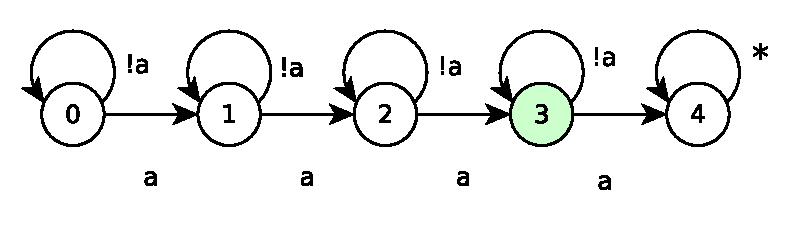
\includegraphics[scale=0.5]{diagrams/threeas.pdf}
        \caption{State machine for input consisting of exactly 3 a's}
        \label{fig:threeas}
    \end{figure}
    
    \item $A = \{a, b, c, d\}$; $S = \{0, 1, 2, 3\}$; machine table: see Table \ref{tab:machine-at-least-3as}; diagram: see Figure \ref{fig:atleast3as}
    \begin{table}[!ht]
        \centering
        \begin{tabular}{l|ll}
        Present state & a & !a \\ \hline
        0             & 1 & 0  \\
        1             & 2 & 1  \\
        2             & 3 & 2  \\
        3             & 4 & 3  \\
        4             & 4 & 4 
        \end{tabular}
        \caption{State machine for input consisting of at least 3 a's}
        \label{tab:machine-at-least-3as}
    \end{table}
    \begin{figure}[!ht]
        \centering
        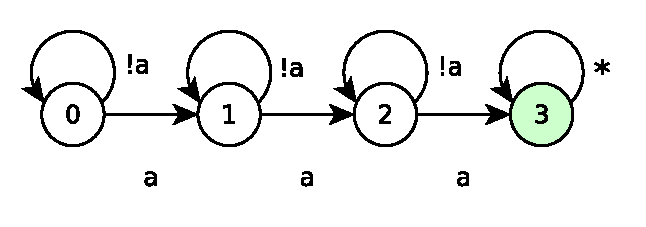
\includegraphics[scale=0.5]{diagrams/atleast3as.pdf}
        \caption{State machine for input consisting of at least 3 a's}
        \label{fig:atleast3as}
    \end{figure}

    \item $A = \{0, 1, 2, 3, 4\}$; $S = \{0, 1, 2, 3, 4\}$; machine table: see Table \ref{tab:add-modulo-5}; diagram: see Figure \ref{fig:add-modulo-5}
    \begin{table}[]
        \centering
        \begin{tabular}{l|lllll}
        Present state & 0 & 1 & 2 & 3 & 4 \\ \hline
        0             & 0 & 1 & 2 & 3 & 4 \\
        1             & 1 & 2 & 3 & 4 & 0 \\
        2             & 2 & 3 & 4 & 0 & 1 \\
        3             & 3 & 4 & 0 & 1 & 2 \\
        4             & 4 & 0 & 1 & 2 & 3
        \end{tabular}
        \caption{State machine for addition modulo 5}
        \label{tab:add-modulo-5}
    \end{table}
    \begin{figure}[!ht]
        \centering
        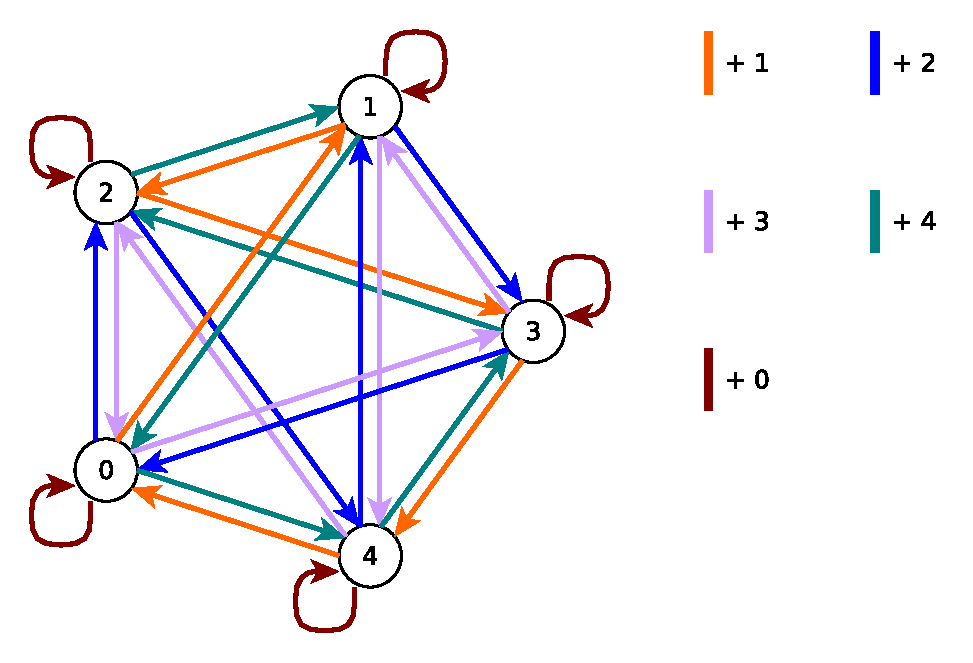
\includegraphics[scale=0.5]{diagrams/add-modulo-5.pdf}
        \caption{State machine for addition modulo 5}
        \label{fig:add-modulo-5}
    \end{figure}

    \item $A = \{0, 1\}$; $S = \{0, 1, 2, 3\}$; machine table: see Table \ref{tab:ends-in-111}; diagram: see Figure \ref{fig:ends-in-111}.
    \begin{table}[]
        \centering
        \begin{tabular}{l|ll}
        Present state & 0 & 1 \\ \hline
        0             & 0 & 1 \\
        1             & 0 & 2 \\
        2             & 0 & 3 \\
        3             & 0 & 0
        \end{tabular}
        \caption{State machine for binary string ending in 111}
        \label{tab:ends-in-111}
    \end{table}
    \begin{figure}[!ht]
        \centering
        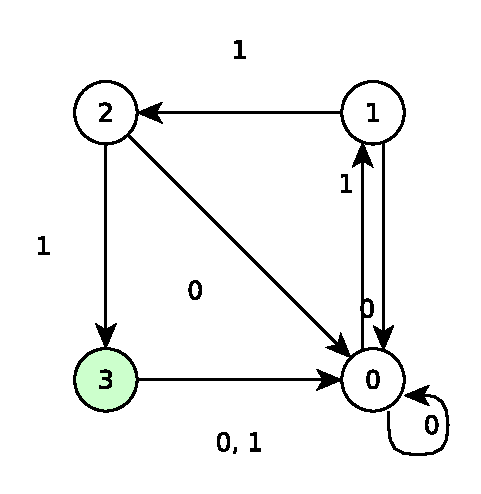
\includegraphics[scale=0.5]{diagrams/ends-in-111.pdf}
        \caption{State machine for binary string ending in 111}
        \label{fig:ends-in-111}
    \end{figure}

    \item \begin{enumerate}[label=(\alph*)]
        \item 
        $\bar{\alpha}(s_0, 000) = s_0$\quad
        $\bar{\alpha}(s_0, 100) = s_1$\\
        $\bar{\alpha}(s_0, 001) = s_1$\quad
        $\bar{\alpha}(s_0, 101) = s_0$\\
        $\bar{\alpha}(s_0, 010) = s_1$\quad
        $\bar{\alpha}(s_0, 110) = s_0$\\
        $\bar{\alpha}(s_0, 011) = s_0$\quad
        $\bar{\alpha}(s_0, 111) = s_1$

        \item 
        $\bar{\alpha}(s_0, 00) = s_0$\quad
        $\bar{\alpha}(s_1, 00) = s_1$\\
        $\bar{\alpha}(s_0, 01) = s_1$\quad
        $\bar{\alpha}(s_1, 01) = s_0$\\
        $\bar{\alpha}(s_0, 10) = s_1$\quad
        $\bar{\alpha}(s_1, 10) = s_0$\\
        $\bar{\alpha}(s_0, 11) = s_0$\quad
        $\bar{\alpha}(s_1, 11) = s_1$
    \end{enumerate}

    \item
        \begin{enumerate}[label=(\alph*)]
            \item 
            $\mathbf{x} = 01001$:\quad $T_\mathbf{x}(s_0) = s_0$\quad $T_\mathbf{x}(s_1) = s_1$\\
            $\mathbf{x} = 10011$:\quad $T_\mathbf{x}(s_0) = s_1$\quad $T_\mathbf{x}(s_1) = s_0$\\
            $\mathbf{x} = 01010$:\quad $T_\mathbf{x}(s_0) = s_0$\quad $T_\mathbf{x}(s_1) = s_1$

            \item In the case of $M_1$, $T_\mathbf{x}$ either maps the initial state to the same state if the weight of $\mathbf{x}$ is even and to the opposite state otherwise. So, there are only two functions.

            \item In general, let $n$ be the number of $a$'s in a given $\mathbf{x}$; then $T_\mathbf{x}(s_i) = s_j$, in which $j = \max(i + n, 4)$.

            \item We can think of $T_\mathbf{x}(s_i)$ as a fuction $f(\mathbf{x}, i) = \sum\limits_{b \in \mathbf{x}} (b \mod 4) + (i \mod 4)$. Since $\mathbf{x}$ determines the function and there are only 5 possible values for the term that includes it in $f$, there are therefore only 5 distinct transition functions in this case.
        \end{enumerate}
\end{enumerate}

\subsection{Set I}
\begin{enumerate}
    \item see Table \ref{tab:automaton-mz4} and Figure \ref{fig:automaton-mz4}.
    
    \begin{table}[]
        \centering
        \begin{tabular}{l|llll}
        Present state & 0 & 1 & 2 & 3 \\ \hline
        0             & 0 & 1 & 2 & 3 \\
        1             & 1 & 2 & 3 & 0 \\
        2             & 2 & 3 & 0 & 1 \\
        3             & 3 & 0 & 1 & 2
        \end{tabular}
        \caption{Automaton $M(\mathbb{Z}_4)$}
        \label{tab:automaton-mz4}
    \end{table}
    \begin{figure}
        \centering
        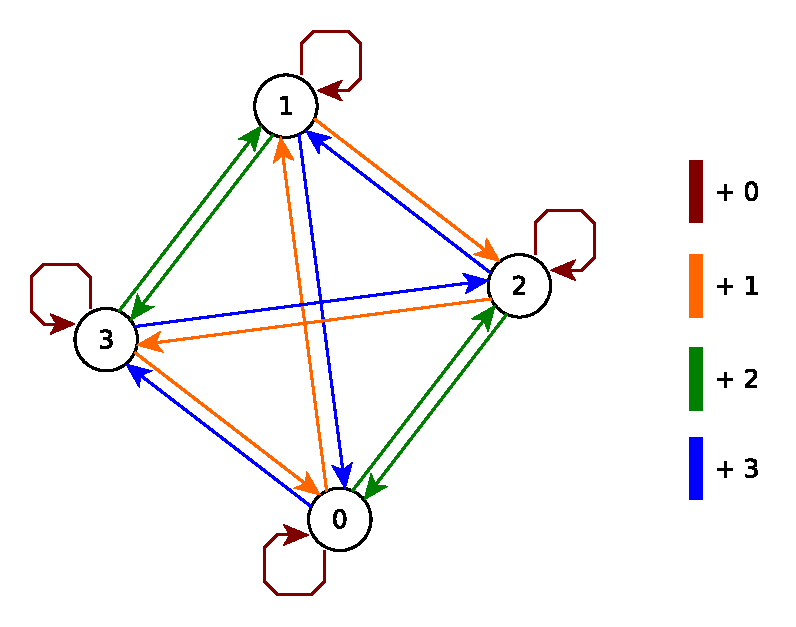
\includegraphics[scale=0.5]{diagrams/automaton-mz4.pdf}
        \caption{Automaton $M(\mathbb{Z}_4)$}
        \label{fig:automaton-mz4}        
    \end{figure}

    \item \begin{minipage}{0.5\textwidth}
        \centering
        $e = \begin{bmatrix}
            1 & 2 & 3 \\
            1 & 2 & 3 \\
        \end{bmatrix}$\\
        $a = \begin{bmatrix}
            1 & 2 & 3 \\
            1 & 3 & 2 \\
        \end{bmatrix}$\\
        $b = \begin{bmatrix}
            1 & 2 & 3 \\
            3 & 1 & 2 \\
        \end{bmatrix}$\\
        $c = \begin{bmatrix}
            1 & 2 & 3 \\
            3 & 2 & 1 \\
        \end{bmatrix}$\\
        $d = \begin{bmatrix}
            1 & 2 & 3 \\
            2 & 3 & 1 \\
        \end{bmatrix}$\\
        $f = \begin{bmatrix}
            1 & 2 & 3 \\
            2 & 1 & 3 \\
        \end{bmatrix}$\\
    \end{minipage}
    \begin{minipage}{0.5\textwidth}
        \centering
        \begin{tabular}{l|llllll}
            $\circ$ & $e$ & $a$ & $b$ & $c$ & $d$ & $f$ \\ \hline
            $e$       & $e$ & $a$ & $b$ & $c$ & $d$ & $f$ \\
            $a$       & $a$ & $e$ & $f$ & $d$ & $c$ & $b$ \\
            $b$       & $b$ & $c$ & $d$ & $f$ & $e$ & $a$ \\
            $c$       & $c$ & $b$ & $a$ & $e$ & $f$ & $d$ \\
            $d$       & $d$ & $f$ & $e$ & $a$ & $b$ & $c$ \\
            $f$       & $f$ & $d$ & $c$ & $b$ & $a$ & $e$
        \end{tabular}
    \end{minipage}\\        
    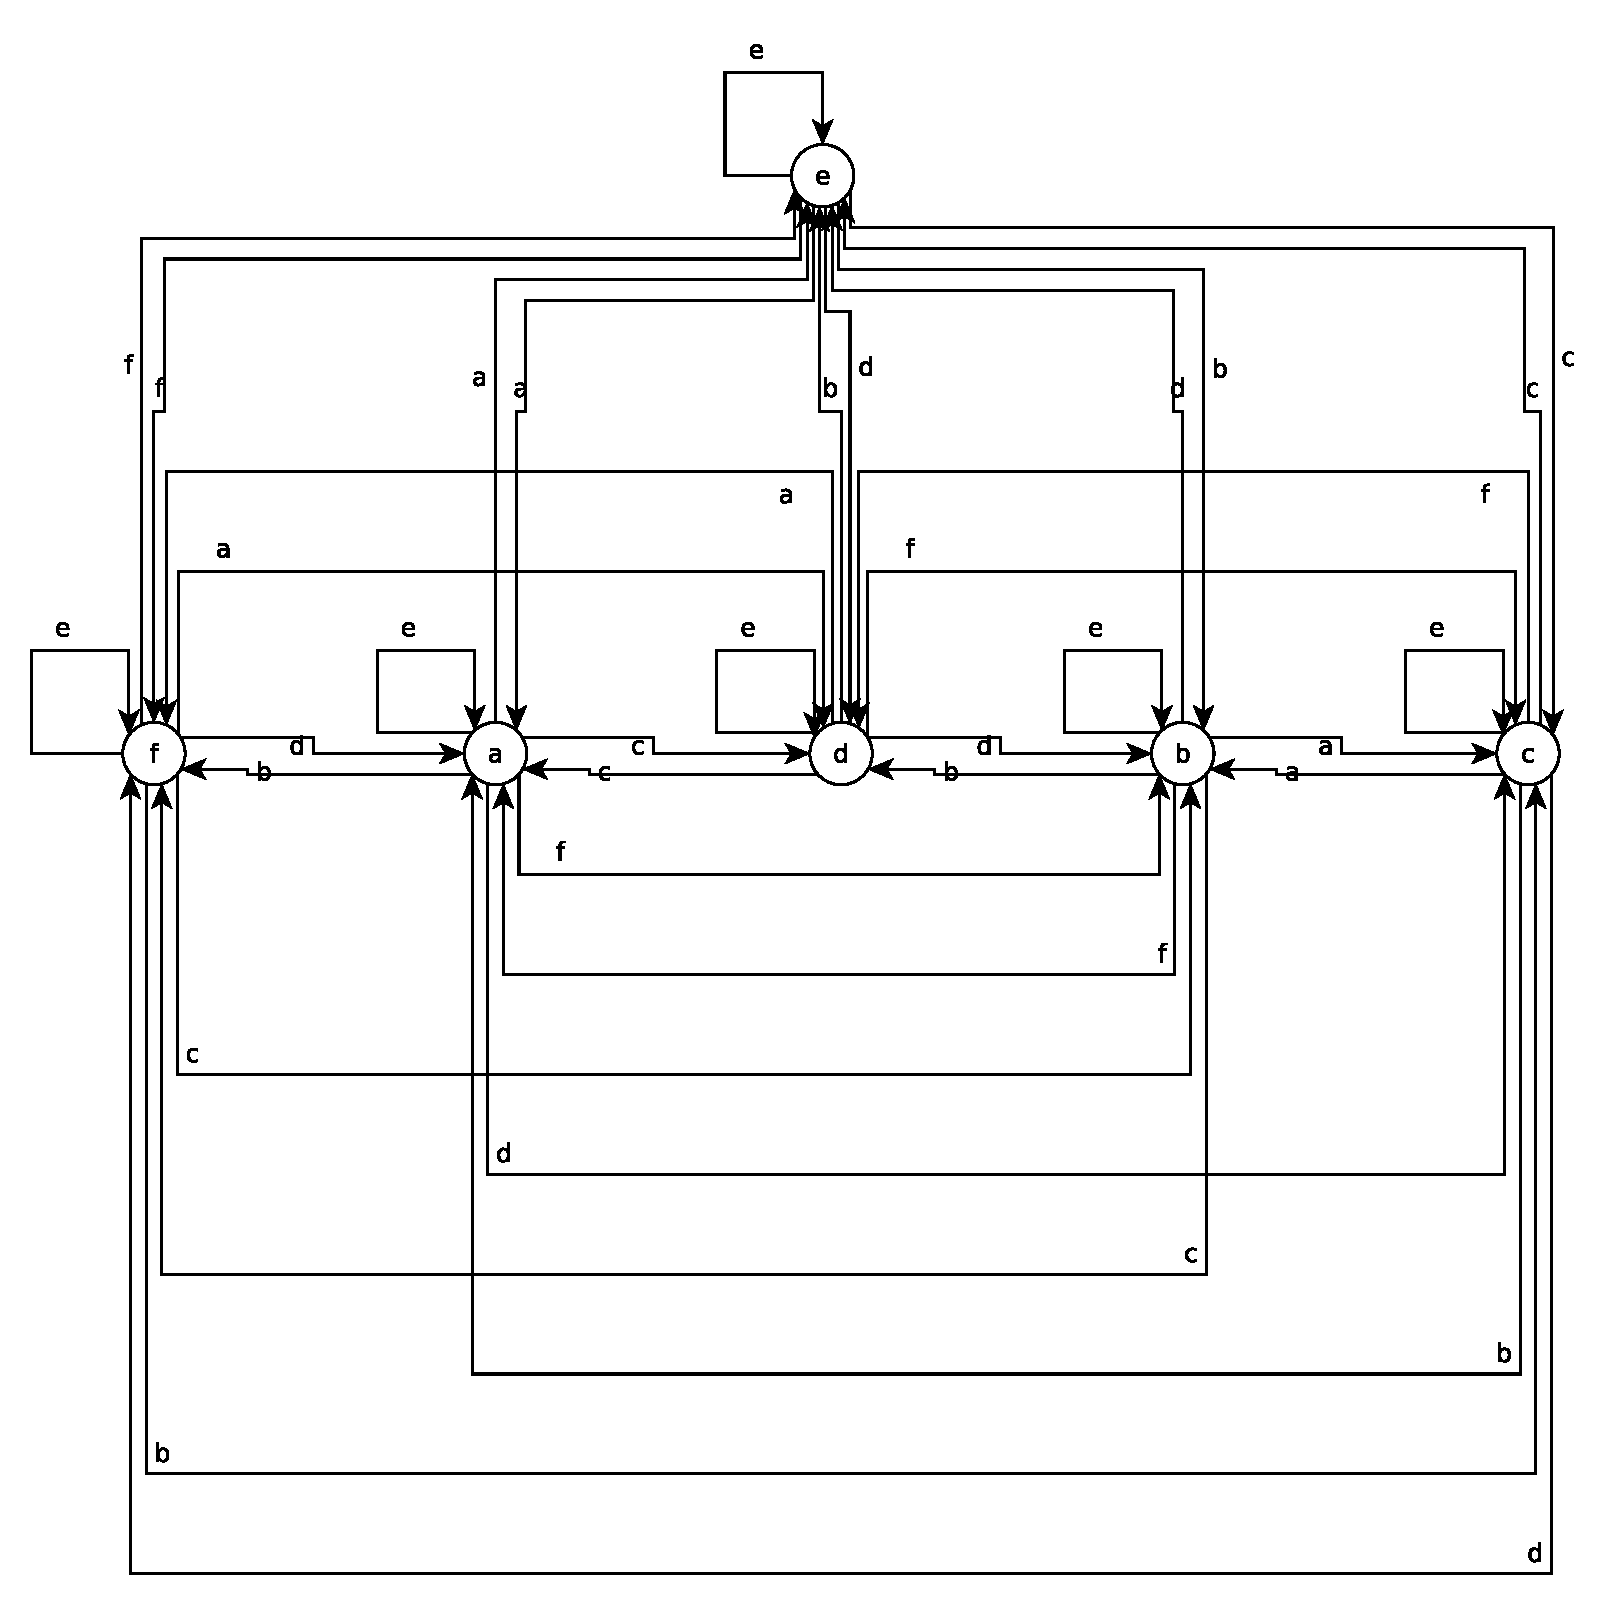
\includegraphics[scale=0.5]{diagrams/automaton-s3.pdf}

    \item $(T_\mathbf{y} \circ T_\mathbf{x})(s_i) = \bar{\alpha}(\bar{\alpha}(s_i, \mathbf{x}), \mathbf{y})$. This corresponds to putting the automaton in the state $s_i$, then applying all the events in $\mathbf{x}$ and then applying all the events in $\mathbf{y}$. Symbolically, $(T_\mathbf{y} \circ T_\mathbf{x})(s_i) = \bar{\alpha}(s_i, \mathbf{xy}) = T_\mathbf{xy}$.

    \item As we've seen in exercise H5b of this chapter, there are only two transition functions for $M_1$. Let us call them $E(s_i) = s_i$ and $I(s_i) = s_{\text{inverse of}\, i}$. See Table \ref{tab:op-semigroup-m1} for the group operation of $\mathscr{S}(M_1)$. $E$ is the identity element and each element is the inverse of itself. So $\mathscr{S}(M_1)$ is also a group.

    \begin{table}[!ht]
        \centering
        \begin{tabular}{l|ll}
        $\circ$ & $E$ & $I$ \\ \hline
        $E$     & $E$ & $I$ \\
        $I$     & $I$ & $E$
        \end{tabular}
        \caption{Operation table of $\mathscr{S}(M_1)$}
        \label{tab:op-semigroup-m1}
    \end{table}
    
    \item As we've seen, there are only 5 transition functions in $M_2$. Let's call them $P_i$, for $0 \leqslant i \leqslant 4$, so that $P_i(s_j) = (i + j) \mod 4$. The operation table is essentially the same as Table \ref{tab:add-modulo-5}. And it is also a group.

    \item \emph{The diagram shows multiple arrows for the same event leaving the same state. This is not a state machine.}
\end{enumerate}

\section{Chapter 7}

\subsection{Set A}

\begin{enumerate}
    \item $f^{-1} = \begin{bmatrix}
        1 & 2 & 3 & 4 & 5 & 6 \\
        2 & 6 & 3 & 5 & 4 & 1 \\
    \end{bmatrix}$\quad
    $g^{-1} = \begin{bmatrix}
        1 & 2 & 3 & 4 & 5 & 6 \\
        3 & 1 & 2 & 6 & 5 & 4 \\
    \end{bmatrix}$\quad
    $h^{-1} = \begin{bmatrix}
        1 & 2 & 3 & 4 & 5 & 6 \\
        2 & 6 & 1 & 4 & 5 & 3 \\
    \end{bmatrix}$\\\\
    $g \circ f = \begin{bmatrix}
        1 & 2 & 3 & 4 & 5 & 6 \\
        4 & 2 & 1 & 5 & 6 & 3 \\
    \end{bmatrix}$\quad
    $f \circ g = \begin{bmatrix}
        1 & 2 & 3 & 4 & 5 & 6 \\
        1 & 3 & 6 & 2 & 4 & 5 \\
    \end{bmatrix}$

    \item $f \circ (g \circ h) = \begin{bmatrix}
        1 & 2 & 3 & 4 & 5 & 6 \\
        6 & 1 & 5 & 2 & 4 & 3 \\
    \end{bmatrix}$

    \item $g \circ h^{-1} = \begin{bmatrix}
        1 & 2 & 3 & 4 & 5 & 6 \\
        3 & 4 & 2 & 6 & 5 & 1 \\
    \end{bmatrix}$

    \item $h \circ g^{-1} \circ f^{-1} = \begin{bmatrix}
        1 & 2 & 3 & 4 & 5 & 6 \\
        3 & 4 & 1 & 5 & 2 & 6 \\
    \end{bmatrix}$

    \item $g \circ g \circ g = \begin{bmatrix}
        1 & 2 & 3 & 4 & 5 & 6 \\
        1 & 2 & 3 & 6 & 5 & 4 \\
    \end{bmatrix}$
\end{enumerate}

\subsection{Set B}

\begin{enumerate}
    \item $G$ is a group since the composition of functions is associative, there is an identity element, $\epsilon$, and each element is its own inverse. Operation table:
    \begin{center}
            \begin{tabular}{l|llll}
            $\circ$       & $\epsilon$ & $f$        & $g$        & $h$           \\\hline
            $\epsilon$    & $\epsilon$ & $f$        & $g$        & $h$           \\
            $f$           & $f$        & $\epsilon$ & $h$        & $g$           \\
            $g$           & $g$        & $h$        & $\epsilon$ & $f$           \\
            $h$           & $h$        & $g$        & $f$        & $\epsilon$
        \end{tabular}
    \end{center}
        
    \item $f = \begin{bmatrix}
        1 & 2 & 3 & 4 & 5 & 6 \\
        2 & 3 & 4 & 1 & 6 & 5 \\
    \end{bmatrix}$\quad
    $f^{2} = \begin{bmatrix}
        1 & 2 & 3 & 4 & 5 & 6 \\
        3 & 4 & 1 & 2 & 5 & 6 \\
    \end{bmatrix}$\quad
    $f^{3} = \begin{bmatrix}
        1 & 2 & 3 & 4 & 5 & 6 \\
        4 & 1 & 2 & 3 & 6 & 5 \\
    \end{bmatrix}$\quad
    $f^{4} = \epsilon = \begin{bmatrix}
        1 & 2 & 3 & 4 & 5 & 6 \\
        1 & 2 & 3 & 4 & 5 & 6 \\
    \end{bmatrix}$

    \item \begin{minipage}{0.5\textwidth}
        \centering
        $e = \begin{bmatrix}
            1 & 2 & 3 & 4 & 5 \\
            1 & 2 & 3 & 4 & 5
        \end{bmatrix}$\\
        $f = \begin{bmatrix}
            1 & 2 & 3 & 4 & 5 \\
            4 & 3 & 2 & 1 & 5
        \end{bmatrix}$\\
        $g = \begin{bmatrix}
            1 & 2 & 3 & 4 & 5 \\
            2 & 1 & 4 & 3 & 5
        \end{bmatrix}$\\
        $h = \begin{bmatrix}
            1 & 2 & 3 & 4 & 5 \\
            3 & 4 & 1 & 2 & 5
        \end{bmatrix}$
    \end{minipage}
    \begin{minipage}{0.5\textwidth}
        \centering
        \begin{tabular}{l|llll}
            $\circ$ & $e$ & $f$ & $g$ & $h$ \\ \hline
            $e$       & $e$ & $f$ & $g$ & $h$ \\
            $f$       & $f$ & $e$ & $h$ & $g$ \\
            $g$       & $g$ & $h$ & $e$ & $f$ \\
            $h$       & $h$ & $g$ & $f$ & $e$
        \end{tabular}            
    \end{minipage}

    \item \textbf{TODO}
\end{enumerate}

\subsection{Set C}
\begin{enumerate}
    \item $f(g(x)) = \frac{1}{(1 - (x - 1) / x)} = x$ and $g(f(x)) = \frac{x/(1 - x)}{1/(1 - x)} = x$. Therefore $A$ is closed under composition and inverses.

    \item Every function is its own inverse and $gf = fg = h$, $fh = hf = g$ and $gh = hg = f$.  Therefore $A$ is closed under composition and inverses.

    \item \textbf{TODO}

    \item \textbf{TODO}
\end{enumerate}

\subsection{Set D}
\begin{enumerate}
    \item $f_n: \mathbb{R} \to \mathbb{R}$ is bijective and its inverse is defined as $f_n^{-1}(x) = x - n$.

    \item $f_n(f_m(x)) = x + m + n = f_{n + m}(x)$. $f_{-n}(f_n(x)) = x + n - n = x$. Therefore $f_{-n} = f^{-1}_n$.

    \item $G$ is closed under composition and inverses (see previous item).

    \item $f_1$ is a generator of $G$.
\end{enumerate}

\subsection{Set E}
\begin{enumerate}
    \item $f_{a,b}: \mathbb{R} \to \mathbb{R}$ is bijective and its inverse is defined as $f_{a,b}^{-1}(x) = (x - b)/a$.

    \item $f_{a,b}(f_{c,d}(x)) = f_{a,b}(cx + d) = a(cx + d) + b = acx + ad + b = f_{ac, ad + b}(x)$.

    \item $f_{a,b}^{-1}(x) = (x - b)/a = (1/a)x - b/a = f_{1/a, -b/a}(x)$.

    \item From the previous item we know that $G$ is closed under composition and inverses.
\end{enumerate}

\subsection{Set F}
\begin{enumerate}
    \item $R_0 = \begin{bmatrix}
        1 & 2 & 3 & 4 & 5 & 6\\
        1 & 2 & 3 & 4 & 5 & 6\\
    \end{bmatrix}$\quad
    $R_1 = \begin{bmatrix}
        1 & 2 & 3 & 4 & 5 & 6\\
        2 & 3 & 4 & 5 & 6 & 1\\
    \end{bmatrix}$\quad
    $R_2 = \begin{bmatrix}
        1 & 2 & 3 & 4 & 5 & 6\\
        3 & 4 & 5 & 6 & 1 & 2\\
    \end{bmatrix}$\\
    $R_3 = \begin{bmatrix}
        1 & 2 & 3 & 4 & 5 & 6\\
        4 & 5 & 6 & 1 & 2 & 3\\
    \end{bmatrix}$\quad
    $R_4 = \begin{bmatrix}
        1 & 2 & 3 & 4 & 5 & 6\\
        5 & 6 & 1 & 2 & 3 & 4\\
    \end{bmatrix}$\quad
    $R_5 = \begin{bmatrix}
        1 & 2 & 3 & 4 & 5 & 6\\
        6 & 1 & 2 & 3 & 4 & 5\\
    \end{bmatrix}$\\
    $R_6 = \begin{bmatrix}
        1 & 2 & 3 & 4 & 5 & 6\\
        5 & 4 & 3 & 2 & 1 & 6\\
    \end{bmatrix}$\quad
    $R_7 = \begin{bmatrix}
        1 & 2 & 3 & 4 & 5 & 6\\
        6 & 5 & 4 & 3 & 2 & 1\\
    \end{bmatrix}$\quad
    $R_8 = \begin{bmatrix}
        1 & 2 & 3 & 4 & 5 & 6\\
        1 & 6 & 5 & 4 & 3 & 2\\
    \end{bmatrix}$\\
    $R_9 = \begin{bmatrix}
        1 & 2 & 3 & 4 & 5 & 6\\
        2 & 1 & 6 & 5 & 4 & 3\\
    \end{bmatrix}$\quad
    $R_{10} = \begin{bmatrix}
        1 & 2 & 3 & 4 & 5 & 6\\
        3 & 2 & 1 & 6 & 5 & 4\\
    \end{bmatrix}$\quad
    $R_{11 }= \begin{bmatrix}
        1 & 2 & 3 & 4 & 5 & 6\\
        4 & 3 & 2 & 1 & 6 & 5\\
    \end{bmatrix}$\quad

    \item \begin{minipage}{0.3\textwidth}
        \centering
        $\epsilon = \begin{bmatrix}
            1 & 2 & 3 & 4\\
            1 & 2 & 3 & 4
        \end{bmatrix}$\\
        $a = \begin{bmatrix}
            1 & 2 & 3 & 4\\
            4 & 3 & 2 & 1
        \end{bmatrix}$\\
        $b = \begin{bmatrix}
            1 & 2 & 3 & 4\\
            2 & 1 & 4 & 3
        \end{bmatrix}$\\
        $c = \begin{bmatrix}
            1 & 2 & 3 & 4\\
            3 & 4 & 1 & 2
        \end{bmatrix}$
    \end{minipage}
    \begin{minipage}{0.6\textwidth}
        \begin{tabular}{l|llll}
            $\circ$ & $\epsilon$ & $a$  & $b$  & $c$  \\\hline
            $\epsilon$     & $\epsilon$ & $a$  & $b$  & $c$  \\
            $a$      & $a$  & $\epsilon$ & $c$  & $b$  \\
            $b$      & $b$  & $c$  & $\epsilon$ & $a$  \\
            $c$      & $c$  & $b$  & $a$  & $\epsilon$
        \end{tabular}
    \end{minipage}

    \item \textbf{TODO}
    
    \item \textbf{TODO}
\end{enumerate}

\subsection{Set G}
\begin{enumerate}
    \item \textbf{TODO}
    \item \textbf{TODO}
    \item \textbf{TODO}
    \item \textbf{TODO}
\end{enumerate}

\subsection{Set H}
\begin{enumerate}
    \item Let $f, g \in G$; then $f(g(a)) = a$, which means that $f \circ g \in G$. And $f(a) = a \Rightarrow f^{-1}(a) = a$, so $f^{-1} \in G$. Therefore $G$ is a subgroup of $S_A$.

    \item Let $f, g \in G$ so that $f$ and $g$ move $n$ and $m$ elements, respectively; then $f \circ g$ can move, at most, a finite number of elements (namely, $n + m$). And $f^{-1}$ maps the same number of elements as $f$. So $G$ is closed under composition and inverses and therefore is a subgroup of $S_A$.

    \item Let $f, g \in G$; then $f(g(x)) \in B$ for any $x \in B$, so $f \circ g \in G$. And let's say $B$ has $n$ elements; then $f$ will map those elements of $B$ to $n$ different elements of $B$ (because $f$ is bijective). $f$ ``exhausts'' all elements of $B$, in the sense that there can be no element in $B$ that is not an image of $B$ under $f$. More formally, for any $x \in A$, $f(x) \in B \Rightarrow x \in B$. So $f^{-1} \in G$. Therefore $G$ is a subgroup of $S_A$.

    \item Let us define a function $f: \mathbb{N} \to \mathbb{N}$ such that $f(n) = 2n$ if $n$ is even; if $n$ is odd, we ``cover the holes'' left by the even integers. So, the function looks like:
        $$
            f = \begin{bmatrix}
                0 & 1 & 2 & 3 & 4 & 5 & 6 & 7 & 8 & \ldots\\
                0 & 1 & 4 & 2 & 8 & 3 & 12 & 5 & 16 & \ldots
            \end{bmatrix}
        $$
    $A = \mathbb{N}$ and $B = \{x \in \mathbb{N}: x = 2k, k \in \mathbb{N}\}$. It is clear that $f$ maps every even number to another even number. Due to the way it is constructed, $n_1 \ne n_2 \Rightarrow f(n_1) \ne f(n_2)$ (injective). The function definition also guarantees that any integer $m$ is the image of some integer $n$; $\mathbb{N}$ is infinite, so if we keep incrementing $x$, eventually it will map to $m$ (surjective). So $f$ is a permutation. But note, for example, that $f^{-1}(2) = 3$. So $f^{-1} \notin G$ and, therefore, $G$ is not a subgroup of $S_A$.
\end{enumerate}

\subsection{Set I}
\begin{enumerate}
    \item $\alpha(k_i) = k_i = \epsilon(k_i)$. From (viii) we can conclude that $\alpha = \epsilon$.

    \item We can think of this group as a directed graph in which the edges are the clans and, for any pair $(k_i, k_j)$, there is a directed vertex $k_i \to k_j$ if, and only if, $\alpha(k_i) = k_j$. This graph must have a cycle since: 1) every edge has an outgoing vertex (it's always possible to apply $\alpha$ to any edge) and 2) the set of clans is finite, so any sufficiently long path will eventually revisit some edge. In fact, the length of any cycle is no greater than $n$ (otherwise, that path would have more than $n$ \emph{different} edges, which is impossible).

    So, take any cycle and any clan $k$ in that cycle. Let $m \leqslant n$ be the length of this cycle. Algebraically, we have $\alpha^m(k) = k = \epsilon(k)$. By (viii), $\alpha^m = \epsilon$.

    \item From (vii) we can conclude that the number of permutations cannot be less than $n$ (otherwise, for any given clan $k_i$ there would be another clan $k_j$ so that people in $k_i$ would not have any relation in $k_j$) and it cannot be greater than $n$ either
     (otherwise it would result in more than $n$ clans, which is impossible). So the number of permutations is exactly $n$.

    \item Let's say people in clan $k_i$ have children in clan $k_j$, that is, $c(k_i) = k_j$. So $c^{-1}(c(k_i)) = k_i = c^{-1} = (k_j)$. In other words, people in $k_j$ have fathers in $c^{-1}(k_j)$. Similarly for $w$.

    \item If $c(k_i) = k_i$ then $c = \epsilon$ by (viii). If a woman is in clan $k_i$, then her husband lives in clan $w^{-1}(k_i)$ and their son lives in clan $c(w^{-1}(k_i)) = k_i = \epsilon(k_i)$. So $c \circ w^{-1} = \epsilon \Rightarrow c = w$.

    \item $c \circ w^{-1} \circ w \circ c^{-1} = \epsilon$, which means that any man and his matrilateral parallel cousins are in the same clan. By (vi), such kind of marriage is prohibited.

    \item \textbf{TODO}.

    \item If a woman is in clan $k_i$ then the son of her mother's brother is in clan $c \circ w \circ c^{-1}(k_i)$. Her husband comes from that clan, so $w^{-1}(k_i) = c \circ w \circ c^{-1}(k_i)$. So $c \circ w \circ c^{-1} = w^{-1}$ and, therefore, $c \circ w = w^{-1} \circ c$.

    \item If a woman is in clan $k_i$ then the son of her father's sister is in clan $c \circ w^{-1} \circ c^{-1}$. Her husband comes from that clan, so $c \circ w^{-1} \circ c^{-1} = w^{-1}$. Therefore $c \circ w^{-1} = w^{-1} \circ c$ .
\end{enumerate}

\section{Chapter 8}
\subsection{Set A}
\begin{enumerate}
    \item
        \begin{enumerate}[label=(\alph*)]
            \item $\begin{bmatrix}
                1 & 2 & 3 & 4 & 5 & 6 & 7 & 8 \\
                4 & 6 & 7 & 5 & 1 & 8 & 3 & 2
            \end{bmatrix}$

            \item $\begin{bmatrix}
                1 & 2 & 3 & 4 & 5 & 6 & 7 & 8 & 9 \\
                7 & 8 & 5 & 9 & 4 & 2 & 1 & 6 & 3
            \end{bmatrix}$

            \item $\begin{bmatrix}
                1 & 2 & 3 & 4 & 5 & 6 & 7 & 8 & 9 \\
                8 & 5 & 6 & 9 & 7 & 3 & 1 & 2 & 4
            \end{bmatrix}$

            \item $\begin{bmatrix}
                1 & 2 & 3 & 4 & 5 & 6 & 7 \\
                2 & 1 & 4 & 7 & 5 & 6 & 3
            \end{bmatrix}$

            \item $\begin{bmatrix}
                1 & 2 & 3 & 4 & 5 & 6 & 7 & 8 \\
                3 & 8 & 2 & 6 & 5 & 1 & 7 & 4 
            \end{bmatrix}$

            \item $\begin{bmatrix}
                1 & 2 & 3 & 4 & 5 & 6 & 7 & 8 & 9 \\
                3 & 5 & 4 & 9 & 2 & 1 & 7 & 6 & 8
            \end{bmatrix}$
        \end{enumerate}

        \item
            \begin{enumerate}[label=(\alph*)]
                \item $(145)(293)(67)$

                \item $(17)(24)(395)(68)$

                \item $(17435)(296)$

                \item $(1928)(375)$
            \end{enumerate}

        \item
            \begin{enumerate}[label=(\alph*)]
                \item $(18)(12)(14)(17)(13)$

                \item $(28)(25)(23)(14)(16)$

                \item $(57)(13)(12)(14)(16)$

                \item $\pi = (76)(58)(12)(14)(13)$
            \end{enumerate}

        \item
            \begin{enumerate}[label=(\alph*)]
                \item $(1,2,4)(3,7)$

                \item $(1,2,5,3,7,4)$
                
                \item $(1,2)(4,7)$
                
                \item $(1,7,3,5)$
                
                \item $(1,4,2,5,3)$
                
                \item $(1,7,4,2,3,5)$
                
                \item $(1,2,4,3,5)$
                
                \item $(1,4,2,7,5)$
            \end{enumerate}

        \item As a cycle: \\
                $(1, 2, 3, 4, 5)$\\
                $(2, 3, 4, 5, 1)$\\
                $(3, 4, 5, 1, 2)$\\
                $(4, 5, 1, 2, 3)$\\
                $(5, 1, 2, 3, 4)$\\\\ 
        As a product of transpositions:\\
        $(1, 5)(1, 4)(1, 3)(1, 2)$\\
        $(1, 5)(1, 4)(1, 3)(1, 2)(3, 4)(4, 3)$\\
        $(1, 5)(1, 4)(1, 3)(1, 2)(3, 5)(5, 3)$\\
        $(1, 5)(1, 4)(1, 3)(1, 2)(3, 2)(2, 3)$\\
        $(1, 5)(1, 4)(1, 3)(1, 2)(3, 1)(1, 3)$\\

        \item
            \begin{enumerate}[label=(\alph*)]
                \item $\alpha = (1, 2, 3)$
                
                \item $\alpha = (1, 4, 2, 5, 3)$
                
                \item $\alpha = (1, 2, 3, 4)$
            \end{enumerate}
\end{enumerate}

\subsection{Set B}
\begin{enumerate}
    \item 
        \begin{enumerate}[label=(\alph*)]
            \item 
                $\alpha^{-1} = (1,3,2)$\\
                $\alpha^2 = (1,3,2)$\\
                $\alpha^3 = ()$\\
                $\alpha^4 = (1,2,3)$\\
                $\alpha^5 = (1,3,2)$
            
            \item 
                $\alpha^{-1} = (1,4,3,2)$\\
                $\alpha^2 = (1,3)(2,4)$\\
                $\alpha^3 = (1,4,3,2)$\\
                $\alpha^4 = ()$\\
                $\alpha^5 = (1,2,3,4)$
            
            \item
                $\alpha^{-1} = (1,6,5,4,3,2)$\\
                $\alpha^2 = (1,3,5)(2,4,6)$\\
                $\alpha^3 = (1,4)(2,5)(3,6)$\\
                $\alpha^4 = (1,5,3)(2,6,4)$\\
                $\alpha^5 = (1,6,5,4,3,2)$    
        \end{enumerate}

    \item Each $\alpha^n$ corresponds to a permutation in which each element maps to the one $n$ ``hops'' ahead in the cycle. More formally, $\alpha^n(a_i) = a_{(i + n) \mod s}$. As a result there are $s$ different powers of $\alpha$.

    \item $\alpha^{-1} = (a_sa_{s - 1}\cdots a_1)$. From the equation in the previous item, $\alpha^{s - 1}(a_i) = a_{(i + s - 1) \mod s}$. So $\alpha^{s - 1}(a_1) = a_s$, $\alpha^{s - 1}(a_2) = a_1$ and so on. So $\alpha^{s - 1} = (a_sa_{s - 1}\cdots a_1) = \alpha^{-1}$.

    \item Let us suppose $s$ is odd. If we start with $a_1$ and keep applying $\alpha^2$ repeatedly, we get $a_3, a_5, \ldots, a_s$, that is, all the elements with odd index. From then on, if we continue applying $\alpha^2$, we get $a_2, a_4, \ldots, a_{s - 1}$, that is, all the elements with even index. With this procedure, we cover all the elements without repeating, thus forming a cycle. Now, if $s$ is even and we apply the same procedure, we only get odd numbers until we eventually return to $a_1$, forming a cycle that does not contain the whole domain (all the evens were left out). So, if $\alpha$ is a cycle, then $s$ is odd.

    \item First, from the equation in item 2, $\alpha^{s + 1}(a_i) = a_{(i + s + 1) \mod s} = a_{(i + 1) \mod s} = \alpha(a_i)$ for any $a_i$ in the domain. So $\alpha = \alpha^{s + 1}$. If $s$ is odd, then $(s + 1)$ is divisible by 2. So, $(\alpha^{(s + 1)/2})^2 = \alpha^{s + 1} = \alpha$.
    
    \item The reasoning here is similar to that in item 4; if $s$ is even and we apply $\alpha^2$ repeatedly starting from $a_1$, we'll generate all elements with odd index and come back to $a_1$, thus forming the cycle $(a_1a_3\ldots a_{s-1})$. Then, if we do the same, but starting from $a_2$, we'll cover all the even indices, forming the cycle $(a_2a_4\ldots a_s)$. These two cycles of length $s/2$ are disjoint and cover the whole domain, so $\alpha^2 = (a_1a_3\ldots a_{s-1})(a_2a_4\ldots a_s)$.

    \item This is a generalization of the previous item; if $s = kt$ and we apply $\alpha^k$ repeatedly starting from $a_1$, we'll generate a cycle $c_1$, composed of the sequence of elements $a_i$ with $i = kj + 1$, for $0 \leqslant j \leqslant t - 1$. Similarly, starting from $a_2$, we generate a cycle $c_2$, composed of the sequence of elements $a_i$ with $i = kj + 2$, for $0 \leqslant j \leqslant t - 1$ and so on until $a_k$. All these cycles of length $s/k$ are disjoint and cover the whole domain, so $a^k = c_1c_2\ldots c_{s/k}$.

    \item Let's start with element $a_i$ and apply $\alpha^n$ repeatedly, generating the sequence $a_i, a_{(i + n)\mod s}, a_{(i + 2n)\mod s}$ and so on. In order for this sequence to form a cycle, for all $0 < j < s$, $jn \mod s$ must be non-zero. Since $\alpha^n = \alpha$, we know that $0 < n < s$. Now, let's assume that there are $j, n$ such that $jn \mod s = 0$, which means that $jn = sk$, for some integer $k$. $s$ cannot be one of the factors of $jn$ ($s$ is greater than both $j$ and $n$). So, if $jn$ can be factored at all, $jn = sk = f_1, f_2, \ldots, k, \ldots, f_m$. Dividing both sides by $k$, we can express $s$ as a product of intergers different from 1 and itself. In other words, $s$ is not prime. Therefore, if $s$ is prime, $\alpha^n$ is a cycle for any integer $n$.
\end{enumerate}

\subsection{Set C}
\begin{enumerate}
    \item Even: (a) and (d) only.

    \item For all subitems, we can start from the same observation: the product of two permutations (each one itself written a product of transpositions) can be represented by the simple concatenation of the two. So the number of transpositions that make up the product is the sum of the number of transpositions in each of the original permutations. Then: 
        \begin{enumerate}
            \item Even plus even is even.
            \item Odd plus odd is even.
            \item Even plus odd is odd.
        \end{enumerate}

    \item Any cycle $(a_1, a_2, \ldots, a_l)$ can be represented as the composition of transpositions $(a_1,a_{l - 1})(a_1,a_{l - 2})\cdots(a_1,a_2)$. So, for a cycle of length $l$, the number of transpositions is $l - 1$. Therefore if $l$ is even, the composition is odd and vice-versa.

    \item 
    \begin{enumerate}
        \item From the previous item, we know that the $\alpha$ can be represented as a product of transpositions with size $l - 1$ and $\beta$ as a product of transpositions with size $m - 1$. And $\alpha\beta$ can be represented as a concatenation of the the these two. Therefore the size of this product is $l + m - 2$.

        \item This is a generalization of item (a).
    \end{enumerate}
\end{enumerate}

\subsection{Set D}
\begin{enumerate}
    \item This is a direct consequence of the fact that disjoint cycles commute.

    \item Let's assume that at least one of $\alpha$ and $\beta$ is not the identity. In this case, $\alpha\beta(x) \ne x$ for all $x \in \{a_1, \ldots, a_s, b_1, \ldots, b_r\}$.

    \item From item 1, $(\alpha\beta)^t = \alpha^t\beta^t$. Since $\alpha$ and $\beta$ are disjoint, so too are $\alpha^t$ and $\beta^t$. From item 2, $\alpha^t = \epsilon$ and $\beta^t = \epsilon$.

    \item $\gamma = (a_sb_1)$, so that $\alpha\beta\gamma = (a_1, \ldots, a_s, b_2, \ldots, b_r, b_1)$.

    \item $\gamma\alpha\beta = (b_2, \ldots, b_r, a_s, a_1, \ldots, a_{s - 1}, b_1)$\\$\alpha\gamma\beta = (a_1, \ldots, a_s, b_1, \ldots, b_r)$.   

    \item \textbf{TODO}
\end{enumerate}

\subsection{Set E}
\begin{enumerate}
    \item $\pi\alpha\pi^{-1}(\pi(a_1)) = \pi\alpha(a_1) = \pi(a_2)$. Analogously for $a_2, \ldots, a_s$.

    \item Let $\alpha = (a_1, \ldots, a_n)$ and $\beta = (b_1, \ldots, b_n)$. Now let's choose any permutation $\pi$ such that $\pi(a_i) = b_i$ for any element in the cycle $\alpha$. Then, we can rewrite $\beta = (\pi(a_1), \ldots, \pi(a_n))$. From the previous item, we know, then, that $\beta = \pi\alpha\pi^{-1}$ and is, therefore, a conjugate of $\alpha$. The same reasoning applies in the other direction.

    \item Let $\alpha = (a_1, \ldots, a_s)$ and $\beta = (b_1, \ldots, b_r)$. Taking any $\pi \in S_n$, $\pi\alpha\pi^{-1} = (\pi(a_1), \ldots, \pi(a_s))$ and $\pi\beta\pi^{-1} = (\pi(b_1), \ldots, \pi(b_r))$. Now suppose $\pi(a_i) = \pi(b_j)$ for some $i, j$. Since $\pi$ is a permutation, $a_i = b_j$, which is false, because $\alpha$ and $\beta$ are disjoint. Therefore $\pi\alpha\pi^{-1}$ and $\pi\beta\pi^{-1}$ are also disjoint.

    \item $\pi\sigma\pi^{-1} = \pi\alpha_1\alpha_2\cdots\alpha_t\pi^{-1} = \pi\alpha_1\pi^{-1}\pi\alpha_2\pi^{-1}\cdots\pi\alpha_t\pi^{-1}$. Each $\pi\alpha_i\pi^{-1}$ is a cycle of the same length of $\alpha_i$ and they are all disjoint (see previous item).

    \item Since $\alpha_1$ and $\alpha_2$ have the same length, it follows (from item 2) that they are conjugate, i.e., there is some permutation $\lambda$ such that $\alpha_1 = \lambda\alpha_2\lambda^{-1}$. Similarly, there is a permutation $\gamma$ such that $\beta_1 = \gamma\beta_2\gamma^{-1}$. Also from item 2, we know that we can construct $\lambda$ in such a way as to map elements in the cycle $\alpha_1$ to elements of $\alpha_2$ (elements from $\beta_1$ are mapped to themselves). Similarly, $\gamma$ maps from elements in $\beta_1$ to elements in $\beta_2$. Since $\alpha_1$ and $\beta_1$ are disjoint, we know (from item 3) that $\alpha_1\beta_1 = \lambda\alpha_2\lambda^{-1}\gamma\beta_2\gamma^{-1}$. But since $\gamma$ and $\lambda$ don't ``modify'' the same elements, we can rewrite the equation as $\alpha_1\beta_1 = \gamma\lambda\alpha_2(\gamma\lambda)^{-1}\gamma\lambda\beta_2(\gamma\lambda)^{-1}$. Making $\pi = \gamma\lambda$, we get $\alpha_1\beta_1 = \pi\alpha_2\beta_2\pi^{-1}$.
\end{enumerate}

\subsection{Set F}
\begin{enumerate}
    \item From exercise 8.B.3, $\alpha^n(a_i) = a_{(i + n) \mod s}$ for any $a_i$ in the cycle. So $\alpha^s(a_i) = a_{(i + s) \mod s} = a_i$ and, therefore, $\alpha^s = \epsilon$. And $\alpha^{2s} = \alpha^s\alpha^s = \epsilon\epsilon = \epsilon$ and $\alpha^{3s} = \alpha^{2s}\alpha^s = \epsilon\epsilon = \epsilon$. $\alpha^k \ne \epsilon$ for all $k < s$, since it will always map an element in the cycle to a different element in the cycle.

    \item This follows straighforwardly from item 1.

    \item
        \begin{enumerate}[label=(\alph*)]
            \item 6
            \item 4
            \item 20
        \end{enumerate}

    \item We need to find the smallest integer $n$ such that $(\alpha\beta)^n = \epsilon$. Since $\alpha$ and $\beta$ commute, $\alpha^n\beta^n = \epsilon$. And since they are disjoint, $\alpha^n = \epsilon$ and $\beta^n = \epsilon$. The order of $\alpha$ is 4, which means that $\alpha^{4p} = \epsilon$ for every integer $p \geqslant 1$. Similarly, the order of $\beta$ is 6, so $\beta^{6q} = \epsilon$ for every integer $q \geqslant 1$. So $n = 4p = 6q$. So the problem now has been reduced to find the least common multiple of 4 and 6, which is 12.

    \item The least common multiple of $r$ and $s$ for the same reasons explained in the previous item.
\end{enumerate}

\subsection{Set G}
\begin{enumerate}
    \item By definition, given any two different permutations $\alpha_i$ and $\alpha_j$, there is some $x$ such that $\alpha_i(x) \ne \alpha_j(x)$. Since $\beta$ is a permutation, there is some $y$ such that $\beta(y) = x$. So $\alpha_i\beta(y) \ne \alpha_j\beta(y)$ and, therefore, $\alpha_1\beta, \ldots, \alpha_r\beta$ are $r$ distinct permutations. That they are odd was already proved in exercise C2.

    \item The proof that they are distinct is the same as in the previous item. That they are even was already proved in exercise C2.

    \item Let's say the number of even permutations in $S_n$ is $r$ and the number of odd permutations is $s$. If we pick any odd permutation and mulitiply by each of the even permutations, we will get $r$ different odd permutations. So $s \geqslant r$. Similarly, if we get any odd permutation and multiply by each of the odd ones (including itself), we get $s$ different even permutations. So $r \geqslant s$. From these two inequalities, we can conclude that $r = s$, that is, the number of odd permutations is equal to the number of even permutations.

    \item From C2, we know that the composition of two even permutations is even; so $A_n$ is closed under composition. And if we reverse the order of the cycles that compose to form a permutation, we get its inverse (that is, $\alpha_1\alpha_2\ldots\alpha_n = (\alpha_n\alpha_{n-1}\ldots\alpha_1)^{-1}$, where $\alpha_i$ are cycles). So, clearly, the inverse of an even permutation is also even, that is $A_n$ is closed under inverses. Therefore $A_n$ is a subgroup of $S_n$.

    \item There are only two possiblities: either $H$ contains only even permutations (of which $A_n$ is an example) or it contains at least one odd permutation. If the former is the case, there is nothing else to prove; if the latter is the case, then we can apply the same reasoning we did in exercise G3, just replacing $S_n$ with $H$.
\end{enumerate}

\subsection{Set H}
\begin{enumerate}
    \item Every permutation can be written as a product of disjoint cycles and every cycle can be written as a product of transpositions. So every permutation can be written as a product of transpositions. In other words, the set of all transpositions in $S_n$ generates $S_n$.

    \item Any cycle $(a_1, a_2, \ldots a_n)$ can be written as the product $(1, a_1)(1, a_n)(1, a_{n-1})\ldots(1, a_1)$. Since any permutation can be written as a product of disjoint cycles, the set $\{(1, a_1), (1, a_2), \ldots (1, a_n)\}$ generates $S_n$.

    \item Every permutation can be written as a product of transpositions of the form $(1, a_i)$ (see exercise H2). Given two elements $x, y$, $(1, x)(1, y) = (1, y, x)$. So we can get any even permutation, and apply this transformation to all consecutive transpositions in the product and the result will be a product of cycles of length 3. Therefore, the set of cycles of length 3 generates $A_n$.
 
    \item \emph{The hint says it all} B-)

    \item \emph{The hint says it all} B-)
\end{enumerate}

\section{Chapter 9}
\subsection{Set A}
\begin{enumerate}
    \item
        \begin{enumerate}
            \item injective: $f(a) = f(b) \Rightarrow \epsilon(a) = \epsilon(b)$.
    
            \item surjective: $f(a) = a$, for every $a \in G$.
    
            \item $f(ab) = \epsilon(ab) = \epsilon(a)\epsilon(b) = f(a)f(b)$.
        \end{enumerate}
    
    \item
        \begin{enumerate}
            \item injective: $f^{-1}(a) = f^{-1}(b) \Rightarrow f(f^{-1}(a)) = f(f^{-1}(b)) \Rightarrow a = b$.
    
            \item surjective: $f^{-1}(f(a)) = a$, for any $a \in G_1$.
    
            \item $f^{-1}(f(a))f^{-1}(f(b)) = ab = f^{-1}(f(ab)) = f^{-1}(f(a)f(b))$, for any $a, b \in G_1$.
        \end{enumerate}
    item
        \begin{enumerate}
            \item injective: $ g(f(a)) = g(f(b)) \Rightarrow f(a) = f(b) \Rightarrow a = b $.
    
            \item surjective: $ g $ is surjective, so for any $ c \in G_3 $ there exists some $ b \in G_2 $ such that $ g(b) = c $. $ f $ is surjective, so for any $ b \in G_2 $ there exists some $ a \in G_1 $ such that $ f(a) = b $. Therefore, for any $ c \in G_3 $ there is some $ a \in G_1 $ such that $ g(f(a)) = c $.
    
            \item $ g(f(ab)) = g(f(a)f(b)) = g(f(a))g(f(b)) $.
        \end{enumerate}
\end{enumerate}

\subsection{Set B}
\begin{enumerate}
    \item For any $ a \in G_1 $, $ f(e_1)f(a) = f(e_1a) = f(a) $, Therefore, $ f(e_1) $ is the neutral element $ e_2 \in G_2 $.
    
    \item $ e_2 = f(e_1) = f(aa^{-1}) =f(a)f(a^{-1}) \Rightarrow f^{-1}(a) = f(a^{-1}) $.
    
    \item Any $ b \in G_1 $ can be written as $ b = a^n $, for some integer $n$. So every element of $ G_2 $ can be written as $ f(a^n) = f^n(a) $.
\end{enumerate}

\subsection{Set C}
\begin{enumerate}
    \item $ G \ncong H $. In $ G $, every element is its own inverse. In $ H $, $ i.i \ne 1 $.
    
    \item $ G \ncong H $. In $ \mathbb{Z}_4 $, $ 1 + 1 = 2 \ne 0 $.
    
    \item $ G \ncong H $. In $ G $, every element is its own inverse. In $ H $, $ i.i \ne 1 $.
    
    \item $ G \cong H $. $ A = (23) $, $ B = (123) $, $ C = (13) $, $ D = (132) $, $ K = (12) $, $ I = () $.
    
    \item \textbf{TODO}.
    
    \item $ G \ncong H $. In $ G $, every element is its own inverse. In $ H $, $ i.i \ne 1 $.
\end{enumerate}

\subsection{Set D}
\begin{enumerate}
    \item $ \mathbb{Z}_2 \times \mathbb{Z}_2 \cong P_2 $. $ f: P_2 \rightarrow \mathbb{Z}_2 \times \mathbb{Z}_2, f = 
    \begin{pmatrix}
        \emptyset & {a}    & {b}    & {a, b}\\
        (0, 0)    & (0, 1) & (1, 0) & (1, 1)
    \end{pmatrix} $.\\
    $ \mathbb{Z}_4 \cong V $. $ f: \mathbb{Z}_4 \rightarrow V, f = 
    \begin{pmatrix}
        0 & 1 &  2 & 3 \\
        1 & i & -1 & -i
    \end{pmatrix}$.
    
    \item $ \mathbb{Z}_3 \times \mathbb{Z}_2 \cong \mathbb{Z}_6 \cong \mathbb{Z}_7^* $. Each of these three groups is generated by a single element: $ (1, 1) $, $ 1 $ and $ 3 $, respectively. $ S_3 $ does not have this property, so it is not isomorphic to the other three groups.
    
    \item $ P_3 $.
    
    \item For this exercise, let's call the groups $ A $, $ B $, $ C $ and $ D $, respectively according to the order in which they appear in the book.

    $ A $ and $ B $ are generated by two elements each. In $ A $, let's call them $ a $ and $ b $. From the diagrams we can deduce that $ a^2 = b^3 = e $. In $ B $, let's call them $ c $ and $ d $. Similarly, $ c^2 = d^3 = e $. If they are to be isomorphic, a necessary condition is: any isomorphism between them maps $ a \to c $ and $ b \to d $. However, $ ba = ab^2 $ and $ dc = cd $. If they were isomorphic, $ dc $ would equal $ cd^2 $.

    $ C $ also has two generators, $ f $ and $ g $. But $ f^2 = g^2 = e $, which is different from $ A $ and $ B $. So $ C $ is not isomorphic to any of them.

    $ D $ has only one generator, so it's not isomorphic to any of the other groups.
\end{enumerate}

\subsection{Set E}
\begin{enumerate}
    \item $ f: \mathbb{Z} \to E, f(n) = 2n $.
        \begin{enumerate}
    
            \item injective: $ f(a) = f(b) \Rightarrow 2a = 2b \Rightarrow a = b $.
    
            \item surjective: by definition, for any $ m \in E $, $ m = 2k $, for some $ k \in \mathbb{Z} $. So $ f(k) = m $.
    
            \item $ f(a) + f(b) = 2a + 2b = 2(a + b) = f(a + b) $.
        \end{enumerate}
    
    \item $ f: \mathbb{Z} \to G, f(n) = 10^n $.
        \begin{enumerate}
    
            \item injective: $ f(a) = f(b) \Rightarrow 10^a = 10^b \Rightarrow a = b $.
    
            \item surjective: For any $ m \in G $, $ f(\log_{10} y) = y $.
    
            \item $ f(a)f(b) = 10^a.10^b = 10^{a + b} = f(a + b) $.
        \end{enumerate}
    
    \item $ f: \mathbb{R} \times \mathbb{R} \to \mathbb{C}, f(a, b) = a + bi $.
        \begin{enumerate}
            \item injective: $ f(a, b) = f(c, d) \Rightarrow a + bi = c + di \Rightarrow a = c, b = d \Rightarrow (a, b) = (c, d) $.

            \item surjective: by definition, for any $ x = a + bi \in \mathbb{C} $, $ f(a, b) = x $, for some pair $ (a, b) \in \mathbb{R} \times \mathbb{R}$.

            \item $ f(a, b) + f(c, d) = (a + bi) + (c + di) = (a + c) + (b + d)i = f(a + c, b + d) $.
        \end{enumerate}

    \item In $ \mathbb{R^*} $, $ -1.(-1) = 1 $, which is the identity element. In other words, $ -1 $ is a non-identity element that is its own inverse. In $ \mathbb{R} $, there is no such element, because $ x + x = 2x $. The only element that satisfies the equation $ 2x = 0 $ is $  x = 0 $. Therefore, $ \mathbb{R^*} \ncong \mathbb{R} $.

    \item $ \mathbb{Z} $ is generated by a single element, $ 1 $. There can be no single element that generates $ \mathbb{Q} $. Let's prove this by contradiction, by assuming there is such a generator $ \frac{a}{b} $. Then, for any other rational number, $ \frac{c}{d} $, there is an integer $ n $ such that $ \frac{a}{b}.n = \frac{c}{d} $. For two rationals to be considered equal, $ and = bc $. Since $ b \ne 0 $, we can rewrite this equation as $ c = \frac{d}{b}an $. That means that all rational numbers whose denominators are not multiples of $ b $ cannot be generated by $ \frac{a}{b} $. Therefore, there is no single generator for $ \mathbb{Q} $ and $ \mathbb{Z} \ncong \mathbb{Q} $. 

    \item Let's assume that there is an isomorphism, $ f: \mathbb{Q} \to \mathbb{Q}^{\mathbf{POS}} $. Being an isomorphism, there must exist some $ a \in \mathbb{Q} $ such that $ f(a) = 2 $. Also,
    $$
        f\left(\frac{a}{2} + \frac{a}{2}\right) = f\left(\frac{a}{2}\right)f\left(\frac{a}{2}\right) = \left[f\left(\frac{a}{2}\right)\right]^2 = 2
    $$

    But there is no element in $ \mathbb{Q}^{\mathbf{POS}} $ whose square is 2. Therefore, there is no isomorphism between $ \mathbb{Q}$ and $\mathbb{Q}^{\mathbf{POS}}$.
\end{enumerate}

\subsection{Set F}
\begin{enumerate}
    \item $ f: G_1 \to G_2 $ is an isomorphism in which $ f((24)) = a $, $ f((1234)) = b $:

    $ (24)^2 = (24)(24) = e $\\
    $ (1234)^4 = (1234)(1234)(1234)(1234) = e $\\
    $ (1234)(24) = (24)(1234)(1234)(1234) = (12)(34) $

    \item  $ f: G \to G' $ is an isomorphism in which $ f((23)) = a $ and $ f((13)) = b $.

    \item \textbf{TODO}

    \item \textbf{TODO}
\end{enumerate}

\subsection{Set G}
\begin{enumerate}
    \item 
        \begin{enumerate}
            \item injective: $ f(a) = f(b) \Rightarrow a - 1 = b - 1 \Rightarrow a = b $.

            \item surjective: For any $ y \in G $, $ f(y + 1) = y $.

            \item $ f(a) * f(b) = a - 1 + b - 1 + ab - a - b + 1 = ab -1 = f(ab) $.
        \end{enumerate}

    \item $ f: \mathbb{R} \to G, f(x) = x - 1 $. This function is bijective for the same reasons shown in the previous exercise. In addition, $ f(a) * f(b) = a - 1 + b - 1 + 1 = a + b - 1 = f(a + b) $.

    \item $ f(x) = 2x $.
        \begin{enumerate}
            \item injective: $ f(a) = f(b) \Rightarrow 2a = 2b \Rightarrow a = b $.

            \item surjective: $ f(y/2) = y$ for any $ y \in G $.

            \item $ f(a) * f(b) = \frac{2a2b}{2} = 2ab = f(ab) $.
        \end{enumerate}

    \item
        \begin{enumerate}
            \item injective: $ f(a, b) = f(c, d) \Rightarrow (-1)^ba = (-1)^dc $. Since $ b $ and $ c $ can only assume the values $ 0 $ and $ 1 $ and $ a $and $ c $ are both positive, we can conclude that $ (a, b) = (c, d) $.

            \item $ f\left(|y|, \frac{-y + |y|}{2|y|} \right) = y $ for any $y \in G$.

            \item $ f(a, b).f(c, d) = (-1)^ab.(-1)^cd = (-1)^{a + c}bd = f(bd, a + c) $. Obs.: in the case $  a = c = 1 $, in $ \mathbb{R}^* $, $ a + c = 2 $ and in $ \mathbb{Z}_2 $, $ a + c = 0 $. But in both cases, $ (-1)^{a + c} = 1 $, so the equality holds.
        \end{enumerate}
\end{enumerate}

\subsection{Set H}
\begin{enumerate}
    \item $ f: G \times H \to H \times G, f(a, b) = (b, a) $ is an isomorphism.
        \begin{enumerate}
            \item $ f(a, b) = f(c, d) \Rightarrow (b, a) = (d, c) \Rightarrow (a, b) = (c, d) $.

            \item surjective: $ f(b, a) = (a, b) $ for any $ (a, b) \in H \times G $.

            \item $ f(a, b)f(c, d) = (b, a)(d, c) = (bd, ac) = f(ac, bd) $.
        \end{enumerate}
    
    \item Let $ g: G_1 \to G_2 $ and $ h: H_1 \to H_2$ be isomophisms. Then $ f(a, b) = (g(a), h(b)) $.
        \begin{enumerate}
            \item injective: $ f(a, b) = f(c, d) \Rightarrow (g(a), h(b)) = (g(c), h(d)) \Rightarrow g(a) = g(c) $  and $ h(b) = h(d) $. Since $ g $ and $ h $ are isomophisms, $ a = c $ and $  b = d $. So $ (a, b) = (c, d) $.

            \item surjective: $ f(g^{-1}(a), h^{-1}(b)) = (a, b) $ for any $ (a, b) \in G _2 \times H_2 $.

            \item $ f(a, b)f(c, d) = (g(a), h(b))(g(c), h(d)) = (g(a)g(c), h(b)h(d)) $. Since $ g $ and $ h $ are isomophisms, $ g(a)g(c) = g(ac) $ and $ h(b)h(d) = h(bd) $. So, $ f(a, b)f(c, d) = (g(ac), h(bd)) = f(ac, bd) $.
        \end{enumerate}

    \item First, let's assume that $ f(x) = x^{-1} $ is an isomorphism from $ G $ to $ G $. Then, for any $ a, b \in G $:
    $$
        f(a)f(b) = f(ab) \Rightarrow a^{-1}b^{-1} = (ab)^{-1} \Rightarrow (ba)^{-1} = (ab)^{-1} \Rightarrow ba = ab
    $$

    Therefore, $ G $ is abelian. To prove the opposite direction, we can simply make the inferences above in the reversse order.

    \item $ f: G \to H, f(x) = x^{-1} $.
        \begin{enumerate}
            \item injective: $ f(a) = f(b) \Rightarrow a^{-1} = b^{-1} \Rightarrow a = b $.

            \item surjective: $ f(y^{-1}) = y $ for any $ y \in H $.

            \item $ f(a) * f(b) =a^{-1} * b^{-1} = b^{-1}a^{-1} = (ab)^{-1} $.
        \end{enumerate}
\end{enumerate}
    
\subsection{Set I}
\begin{enumerate}
    \item Since all elements of $ \mathbb{Z}_6 $ appear in the second row without repetition, $ f $ is bijective. $ f $ can be written as $ f(x) -x $. So,
    $$
        f(a) + f(b) = -a + (-b) = -(a + b) = f(a + b)
    $$

    \item $ f_3(x) = -x $. This is an automorphism for the same reason as the previous item.

    $ f_1(x) = 2x $. $ f_1(a) + f_1(b) = 2a + 2b = 2(a + b) = f(a + b) $.

    $ f_2(x) = 3x $. $ f_1(a) + f_1(b) = 3a + 3b = 3(a + b) = f(a + b) $.

    \item
        \begin{enumerate}
            \item injective: $ f(x) = f(y) \Rightarrow axa^{-1} = aya^{-1} \Rightarrow x = y $.

            \item $ f(a^{-1}ya) = y$ for any $ y \in G $.

            \item $ f(x)f(y) = axa^{-1}aya^{-1} = axya^{-1} = f(xy) $.
        \end{enumerate}

    \item
        For any $ z \in G $ there is a $ y \in G $ such that $ g(y) = z $ because $ g $ is an automorphism.\\
        For any $ y \in G $ there is a $ x \in G $ such that $ f(x) = y $ because $ f$ is an automorphism.\\
        Therefore, for any $ z \in G $ there is a $ x $ such that $ f(g(x)) = z $.

        So, $ \text{Aut}(G) $ is closed under composition. From exercise 9.A.2 we know that if $ f $ is an isomophism, then $ f^{-1} $ is also an isomophism. So $\text{Aut}(G)$ is also closed under inverses. Therefore, $\text{Aut}(G)$ is a subgroup of $ S_G $.
\end{enumerate}

\section{Chapter 10}
\subsection{Set A}
\begin{enumerate}
    \item
        \begin{enumerate}
            \item $ a^ma^n = a^0a^n = ea^n  = a^n = a^{0 + n} = a^{m + n} $.
            
            \item $ m = -p $ for some $  p > 0 $. So,

            $ a^m = a^{-p} = (a^{-1})^p $

            $ a^n = (a^{-1})^{-n} $

            Therefore, $ a^ma^n = (a^{-1})^p(a^{-1})^{-n} = (a^{-1})^{p - n} = a^{-p + n} = a^{m + n} $.

            \item $ m = -k $, $ n = -l $, for some $ k, l > 0 $. So,

            $ a^m = a^{-k} = (a^{-1})^k $

            $ a^n = a^{-l} = (a^{-1})^l $

            Therefore, $ a^ma^n = (a^{-1})^k(a^{-1})^l = (a^{-1})^{k + l} = a^{-(k + l)} = a^{m + n} $.
        \end{enumerate}

    \item
        \begin{enumerate}
            \item $ (a^m)^n = (a^0)^n = e^n = e = e^{0n} = e^{mn} $.

            \item $ (a^m)^n = (a^m)^0 = e = e^{0n} = e^{mn} $.

            \item $ m = -p $ for some $  p > 0 $. So,
            
            $ (a^{m})^n = (a^{-p})^n = ((a^{-1})^p)^n = \underbrace{\underbrace{a^{-1}\ldots a^{-1}}_{\text{$p$ times}}\ldots \underbrace{a^{-1}\ldots a^{-1}}_{\text{$p$ times}}}_{\text{$n$ times}} = (a^{-1})^{pn} = a^{-pn} = a^{mn} $.

            \item $ n = -q $, for some $ q > 0 $.
            
            $ (a^m)^n = (a^m)^{-q} = ((a^m)^{-1})^q = ((a^{-1})^m)^q $. Doing the same transformations as above, we get that $ (a^m)^n = a^{mn} $.

            \item $ m = -p $, $ n = -q $ for some $  p, q > 0 $. So,

            $ (a^m)^n = (a^{-p})^{-q} = ((a^{-p})^{-1})^{q} = (a^{p})^{q} = a^{pq} = a^{mn} $.
        \end{enumerate}

    \item
        \begin{enumerate}
            \item $ (a^n)^{-1} = (a^0)^{-1} = e^{-1} = e = a^{0.-1} = a^{n.-1} = a^{-n}$.

            \item $ (a^n)^{-1} = (a^{-q})^{-1} = a^q = a^{-n}$.
        \end{enumerate}
\end{enumerate}

\subsection{Set B}
\begin{enumerate}
    \item $ \ord(10) = 5 $, because $ 10.1 = 10 $, $ 10.2 = 20 $, $ 10.3 = 5 $, $ 10.4 = 15 $ and $ 10.5 = 0 $.

    \item $ \ord(6) = 8 $, becaue $ 6.1 = 6 $, $ 6.2 = 12 $, $ 6.3 = 2 $, $ 6.4 = 8 $, $ 6.5 = 14 $, $ 6.6 = 4 $, $ 6.7 = 10 $ and $ 6.8 = 0 $.

    \item $ \ord(f) = 4 $. Same process as above.

    \item $ \ord(1) = 1 $ in $ \mathbb{R}^* $. $ \ord(1) = \infty $ in $ \mathbb{R} $.

    \item $$ f^2(x) = \frac{\frac{x}{2-x}}{2 - \left(\frac{x}{2 - x}\right)} = \frac{\frac{x}{2-x}}{\frac{2(2 - x) - x}{2 - x}} = \frac{x}{2(2 - x) - x} $$

    In general, the numerator will stay the same and the denominator can be described by the following recursive function:

    $$
        d^n(x) = 2d^{n - 1}(x) - x
    $$
    
    The non-recursive version of this function is:

    $$
        d^n(x) = 2^n(1 - x) + x
    $$

    Let's prove this by induction. For the base case ($ n = 1 $), we have:

    $$ 
        d^1(x) = 2^1(1 - x) + x = 2 - 2x + x = 2 - x
    $$

    For the induction step, assume that $ d^n(x) = 2^n(1 - x) + x $. Then:
    
    $$ d^{n + 1}(x) = 2(2^n(1 - x) + x) - x = 2^{n + 1} + 2x - x = 2^{n + 1}(1 - x) + x $$

    Thus,

    $$ f^n(x) = \frac{x}{d^n(x)} = \frac{x}{2^n(1 - x) + x} $$
    
    In order for $ f^n(x) = x $ for any $ x \in A $, $ d^n(x) = 1 $ for any $ x \in A $. So,

    $$ 
        2^n(1 - x) + x = 1 \Rightarrow 2^n(1 - x) = 1 - x \Rightarrow 2^n = 1 \Rightarrow n = 0
    $$

    Since the only solution to the equation is $ n = 0 $, $ \ord(f) = \infty$.

    \item Yes, in every group (finite or infinite), $ \ord(e) = 1 $. 

    \item
        \begin{enumerate}
            \item 12

            \item 8, 16

            \item 6, 18

            \item 4, 20
        \end{enumerate}
\end{enumerate}

\subsection{Set C}
\begin{enumerate}
    \item $ \ord(a) = 1 \Rightarrow a^1 = e \Rightarrow a = e $. Conversely, $ e^1 = e \Rightarrow \ord(e) = 1 $.

    \item $ a^{n - r} = a^na^{-r} = ea^{-r} = a^{-r} = (a^r)^{-1} $.

    \item Let's say $ \ord(a) = n $. Then, $ nm = k $, for some integer $ m $. Since $ k $ is odd, it can be written as $ k = 2p + 1 $ for some integer $ p $. Let's assume $ n $ is even, which means it can be written as $ n = 2q $ for some integer $ q $. Replacing all the variables:

    $$ nm = k \Rightarrow 2qm = 2p + 1 $$
    which is impossible. Therefore, $ \ord(a) $ is odd.

    \item Let's say $ \ord(bab^{-1}) = n $. Then, $ \underbrace{bab^{-1}\ldots bab^{-1}}_\text{$n$ times} = ba^nb^{-1} = e $. Multiplying both sides on the left by $ b^{-1} $ and on the right by $ b $: $ a^n = e $. Now let's assume there is another integer $ m < n$ such that $ a^m = e $. Then $ ba^mb^{-1} = e $, contradicting our premise that $ \ord(bab^{-1}) = n. $ So $ n $ is the smallest exponent of $ a $ to yield $ e $ and, therefore, $ \ord(a) = n = \ord(bab^{-1}) $.

    \item Let's say $ \ord(a) = n $. Then $ a^n = e \Rightarrow a^na^{-n} = a^{-n} \Rightarrow (a^{-1})^n = e$. Also, $ n $ is the smallest positive power of $ a $ that is equal to $ e $ for an analogous reason given in the previous exercise.

    \item This is a generalization of the previous two exercises. The proof follows the same pattern.
\end{enumerate}

\subsection{Set D}
\begin{enumerate}
    \item Let $ \ord(a) = n $. Then $ p = nk $ for some integer $ k $ (by theorem 5 of the chapter). Since $ a \ne e $, $ n \ne  1$. Because $ p $ is prime, $  k = 1 $ and, therefore $ p = n $.

    \item Let $ \ord(a) = n $. Then $ (a^k)^n = (a^n)^k = e^k = e $. By theorem 5, we know that $ n $ is a multiple of the order of $ a^k $.

    \item $ km $ is the smallest positive exponent of $ a $ that yields $ e $. It may be possible to rewrite $ km $ as a different product of two integers, but if we fix $ k $, then the other number cannot be smaller than $ m $. Therefore, $ m $ is the smallest exponent of $ a^k $ that yields $ e $, that is, $ \ord(a^k) = m $.

    \item Let's first consider the case in which $ a \ne e $. By the definition of odd number, $ n = 2k + 1 $ for some integer $ k $. So, 
    $$ e = a^{2k + 1} = a^{2k}a \Rightarrow (a^2)^k = a^{-1} \Rightarrow \ord(a^2) \ne k $$

    By theorem 5, the next exponent that yields $e$ is $ 2n $. So, $ (a^{2})^n = e \Rightarrow \ord(a^2) = n $.

    In the case in which $ a = e $, $ \ord(a^2) = \ord(a) = 1 $.

    \item $ a^n = a^{r - s} = e $. By theorem 5, $ n $ is a multiple of $ r - s $.

    \item Let's start by denying the conclusion and assuming that $ a $ is not in the center of $ G $, that is, there is some integer $ x $ such that $ ax \ne xa $. Thus, $ a \ne xax^{-1} $. But we know that $ \ord(a) = \ord(xax^{-1}) = k $, which means that $ a $ is not the only element in $ G $ that has order $ k $ (i.e., there are at least two: $ a $ and $ xax^{-1} $).

    \item Again, let's deny the conclusion by assuming that $ \ord(a^k) = mp $ for some integer $ p $. By part 2, we also know that $ \ord(a^k)q = \ord(a) $ for some integer $ q $. So, $ mpq = \ord(a) $, contradicting the hypothesis.

    \item $ a^{mk} = e $ and $ a^{rk} = e $. By theorem 5, $ mkp = rk $ for some integer $ p $. Dividing by $ k $ on both sides: $ mp = r $. 
\end{enumerate}

\subsection{Set E}
\begin{enumerate}
    \item By theorem 5, $ a^{np} = b^{mq} = e $ for any positive integers $ p, q $. As a consequence, $ a^{np}b^{mq} = e $. If we choose $ p $ and $ q $ such that $ np = mq = k $, then $ (ab)^k = e $ (because $ a $ and $ b $ commute). By definition, the smallest value of $ k $ is $ \lcm(m, n) $. Therefore, $ \ord(ab) = \lcm(m, n) $.    

    \item Let's assume that there exist positive integers $ k, l $ such that $ a^k = b^l \ne e $. Then $ \ord(a^k) = \ord(b^l) \ne 1 $. By exercise D2, we know that there exist positive integers $ p, q $ such that:

    $$ \ord(a^k)p = m $$
    $$ \ord(b^l)q = n $$

    So $ m $ and $ n $ have a common divisor, $ \ord(a^k) = \ord(b^l) $, different from $ \pm 1 $. In other words, they are not relatively prime.

    \item Let's assume there are $ i, j, k, l $ such that $ i \ne k $, $ j \ne l $ and $ a^ib^j = a^kb^l $. Then $ a^{k - i} = b^{j -l} $. From the previous exercise we can conclude that $ m $ and $ n $ are not relatively prime.

    \item For some positive integer $ k $:
        \begin{align*}
            \ord(ab)k &= \lcm(m, n) && \text{by part 1} \\
            \ord(ab)k &= mn && \text{because $ m $ and $ n $ are relatively prime} \\
            (ab)^{mn} &= e && \text{by theorem 5}
        \end{align*}

        Let's assume that there is a positive integer $ p $ such that $  p < m $ and $ (ab)^p = e$. Then

        \begin{align*}
            e = (ab)^p &= a^pb^p && \text{because $ a $ and $ b $ commute} \\
            a^p &= b^{-p}
        \end{align*}

        which contradicts the conclusion of part 2. Therefore $ mn $ is the order of $ ab $.

    \item $ \ord(a) = m = \gcd(m, n)p $ for some integer $ p $. So $ \ord(a^{\gcd(m, n)}) = p $. Since $ a^{\gcd(m, n)} $ and $ b $ commute and $ p $ is relatively prime to $ n $:

    $$ \ord(a^{gcd(m, n)}b) = pn = \frac{m}{\gcd(m, n)}n = \lcm(m, n) $$

    Therefore, $ c = a^{gcd(m, n)}b $.

    \item Consider the group of matrices in page 29 of the book. $ A $ and $ B $ do not commute, $ \ord(A) = 2 $, $ \ord(B) = 3 $ and $ \ord(AB) = \ord(C) = 2 \ne 6 = \lcm(2, 3) $.
\end{enumerate}

\subsection{Set F}
\begin{enumerate}
    \item By theorem 5, $ a $ to the power of every multiple of $ 12 $ is equal to $ e $. So what we are looking for is the smallest multiple of $ 8 $ that is equal to some multiple of $ n $. In other words, we are looking for the positive integer $ k $ such that $ 8k = \lcm(8, 12) = 24 $. Therefore $ k = 3 $.

    \item $ \ord(a) = 12 = 4.3 $. By exercise D3, $ \ord(a^4) = 3 $. Since $ 3 $ is odd, by exercise D4, $ \ord((a^4)^2) = \ord(a^8) = 3 $.

    \item Let $ \ord(a) = n $. Generalizing exercise F1, to find the order of $ a^k $ corresponds to finding the smallest $ j $ such that $ (a^k)^j = a^{kj} = e $. By theorem 5 we know that $ a^{in} = e$ for every positive integer $ i $. So we need to find $ j $ such that $ kj = \lcm(k, n) $. Then:

    $$ \ord(a^k) = j = \frac{\lcm(k, n)}{k} = \frac{kn}{\gcd(k, n)k} = \frac{n}{\gcd(k, n)} = \frac{\ord(a)}{\gcd(k, \ord(a))} $$

    Using this result, we can calculate $ \ord(a^9) = 4 $, $ \ord(a^{10}) = 6 $, $ \ord(a^5) = 12 $.

    \item $5$, $7$ and $11$.

    \item Already proved in exercise F3.

    \item For all values of $ k $ that are relatively prime to $ \ord(a) $.
\end{enumerate}

\subsection{Set G}
\begin{enumerate}
    \item By exercise F3:

    $$ \ord(a^m) = \frac{n}{\gcd(m, n)} = \frac{n}{1} = n$$

    \item $$ n = \frac{n}{\gcd(m, n)} \Rightarrow \gcd(m, n) = 1$$

    \item Because $ k $ is the order of $ a^m $.

    \item By theorem 5, $ t = \frac{n}{\gcd(m, n)}p $ for some positive integer $ p $. Then:

    $$ mt = \frac{m}{\gcd(m, n)}np $$ 

    Since $ \frac{m}{\gcd(m, n)} $ is an integer, $ n $ is a factor of $ mt $.

    \item Already proved in exercise F3.
\end{enumerate}

\subsection{Set H}
\begin{enumerate}
    \item $ \ord(b^3) = \frac{\ord(b)}{\gcd(3, \ord(b))} = 12 \Rightarrow \ord(b) = 12.\gcd(3, \ord(b)) $. Because $ 3 $ is prime, $ \gcd(3, \ord(b)) $ is either $ 1 $ or $ 3 $. Let's assume it's $ 1 $; then $ \ord(b) = 12 $. But $ \gcd(3, 12) = 3 $, contradicting this hypothesis. So, $ \ord(b) = 36 $.

    \item Following the same reasoning above, $ \ord(b) = 24 $.

    \item Following the same reasoning above, $ \ord(b) = 60 $.

    \item $ \ord(b^k) = \frac{\lcm(k, \ord(b))}{k} = n \Rightarrow \lcm(k, \ord(b)) = l\ord(b) = nk $ for some positive integer $ l $. Therefore the order of $ b $ is a factor of $ nk $.

    \item $ b^{n'k}  = e$. For the same reason, $ b^{nk} = e $. So $ b^{n'k} = b^{nk} \Rightarrow n = n' $, which is a contradiction.

    \item $ \ord(b) = \frac{nk}{l} $, in which $ n $ and $ l $ are relatively prime. If $ l > 1 $, it is not a factor of $ n $ and therefore it's not a prime factor of $ k $. In this case, $ l $ does not divide either $ k $ or $ n $. But $ \ord(b) $ is an integer, so $ l = 1 $ and $ \ord(b) = nk $.
\end{enumerate}

\section{Chapter 11}
\subsection{Set A}
\begin{enumerate}
    \item $ \angled{6} = \{0, 6, 12, 2, 8, 14, 4, 10\} $

    \item $ \angled{f} =  \{(), (1642), (14)(26), (1246)\} $

    \item $ \angled{\frac{1}{2}} = \{x \in \mathbb{R}^* : x = \frac{1}{2^i},  i \in \mathbb{Z} \} $; $ \angled{\frac{1}{2}} = \{x \in \mathbb{R} : x = \frac{i}{2}, i \in \mathbb{Z}\}$

    \item $ \angled{f} = \{g \in S_\mathbb{R} : g(x) = x + i, i \in \mathbb{Z}\} $

    \item $ \angled{f} = \{g \in \mathscr{F}(\mathbb{R}) : g(x) = x + i, i \in \mathbb{Z}\} $

    \item Every element $ n \in \mathbb{Z} $ can be written as $ n = 1.n = (-1)(-n) $. Let's say $ a \ne \pm 1 \in \mathbb{Z} $ is a generator of $ \mathbb{Z} $. Then, for any $ n_1, n_2 \in \mathbb{Z} $, $ n_1 = ap_1 $ and $ n_2 = ap_2 $ for some integers $ p_1, p_2 $. In this case, any two different integers would have a common divisor different from $ \pm 1 $, which is clearly not the case. So $ 1 $ and $ -1 $ are the only generators of $ \mathbb{Z} $. Every infinite cyclic group is isomorphic to $ \mathbb{Z} $. So, only $ a $ and $ a^{-1} $ are the generators of $ \angled{a} $.

    \item By Cantor's diagonal argument, there is no bijective function from $ \mathbb{R^*} $ to $ \mathbb{Z} $. Therefore $ \mathbb{R^*} $ is not cyclic.
\end{enumerate}

\subsection{Set B}
\begin{enumerate}
    \item $ G $ has an element of order $ n $. Then, by theorem 3 of chapter 10, $ G $ has $ n $ different elements.

    $ G $ has order $ n $ and is generated by $ a $. Then there exist $ n $ different powers of $ a $ and, therefore, $ \ord(a) = n$.

    \item Let $ G $ be a cyclic group generated by $ a $ and let $ b, c \in G $. Then $ b = a^i $ and $ c = a^j $ for some positive integers $ i, j $. So $ bc = a^ia^j = a^ja^i = cb $.

    \item $ b = a^k $ for some positive integer $ k $, which implies that $ \ord(b) = \ord(a^k) $. By exercise 10.D.2, the order of $ a^k $ (and therefore the order of $ b $) is a factor of the order of $ a $.

    \item If $ k $ divides $ n $ then there is some integer $ p $ such that $ n = pk $. Let $ a $ be the generator of the group. So $ \ord(a) = ord(pk) $ and, therefore, $ \ord(a^p) = k $.

    \item Let $ a, b \in G $ such that $ \ord(a) = m $ and $ \ord(b) = n $. Then $ \ord(ab) = mn $, because $ m $ and $ n $ are relatively prime and $ a $ and $ b $ commute ($ G $ is abelian). Since the order of $ G $ is $ mn $, $ ab $ is its generator and, therefore, $ G $ is cyclic.

    \item Let $ b, c \in \angled{a} $. Then $ b = a^i $  and $ c = a^j $ for some integers $ i, j $. So $ f(b) = f(c) \Rightarrow    a^{im} = a^{jm} \Rightarrow i = j \Rightarrow b = c$. So $ f $ is an injective function. Since domain and codomain are the same in this case, it's also surjective.

    In addition, $ f(a)f(b) = a^mb^m  = (ab)^m = f(ab) $. Therefore, $ f $ is an automorphism.
\end{enumerate}

\end{document}  